%! tex root = ../master.tex

\newcommand{\excreturn}{EXC\_RETURN}

\chapter{System Implementation}
This chapter deals with how the system\textquotesingle s functionalities 
are implemented. Diagrams will be included when necessary, as well as code 
snippets for the interesting parts of the program. In the end, all these
will be reviewed and compared with the actual requirements of the standard.

\section{Hardware}
The Mini-M4 board is a development board, which means that beside the 
microcontroller, it also contains two crystal oscillators, two LEDs, a reset 
button and the peripherals for regulating the power it gets from
a micro-USB connector.
Some of the GPIOs are break through using external pins.
These pins are soldered to the board, and this is setup on a breadboard
for practicality, as seen in \ref{fig:photo1}.

\begin{figure}[H]
\begin{subfigure}{0.5\textwidth}
  \centering
  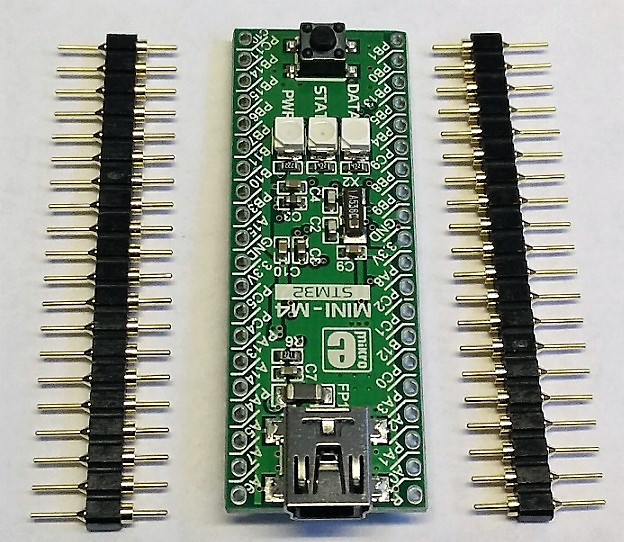
\includegraphics[width=3cm]{hardware/board_not_soldered}
  \caption{MINI-M4 before soldering}
  \label{fig:sub1}
\end{subfigure}%
\begin{subfigure}{0.5\textwidth}
  \centering
  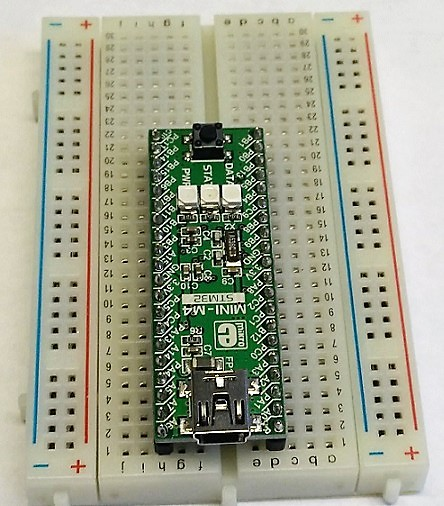
\includegraphics[width=3cm]{hardware/board_on_breadboard}
  \caption{MINI-M4 on a breadboard}
  \label{fig:sub2}
\end{subfigure}
\caption{Preparation of the board}
\label{fig:photo1}
\end{figure}

The JTAG connector is wired to the five corresponding pins of the
board. The serial communication is established with two other wires, going
to the UART pins of the board.
The final setup can be seen in the next figures.

\begin{figure}[H]
\centering
\begin{subfigure}{.5\textwidth}
  \centering
  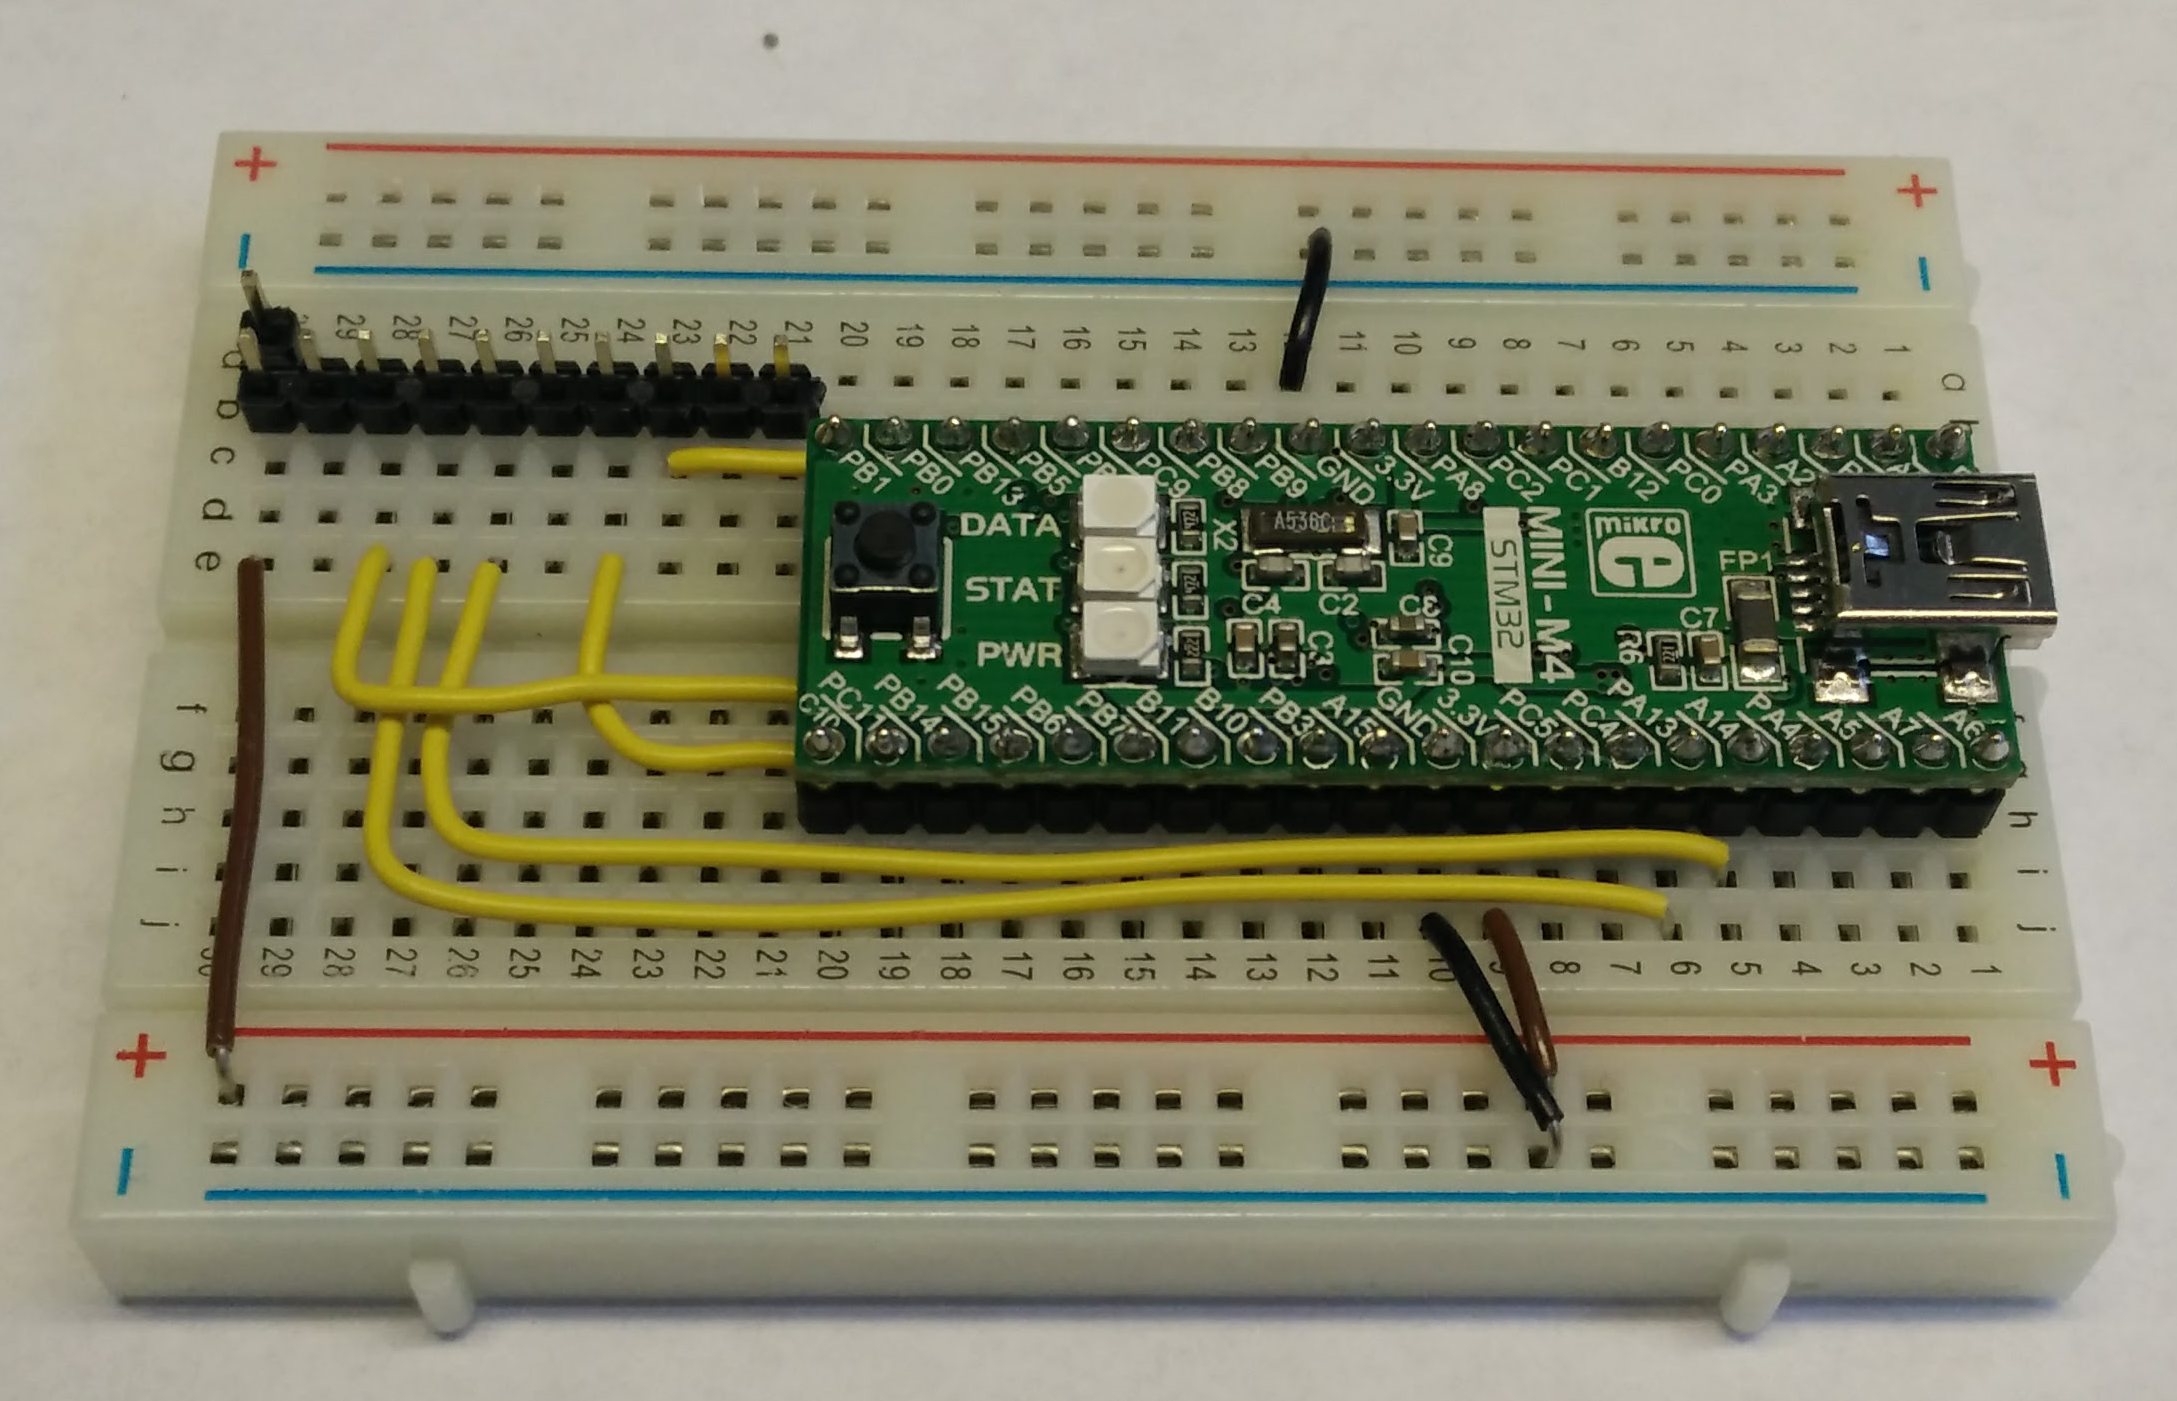
\includegraphics[width=.4\linewidth]{hardware/board_with_jtag_lines}
  \caption{The JTAG lines}
  \label{fig:sub1}
\end{subfigure}%
\begin{subfigure}{.5\textwidth}
  \centering
  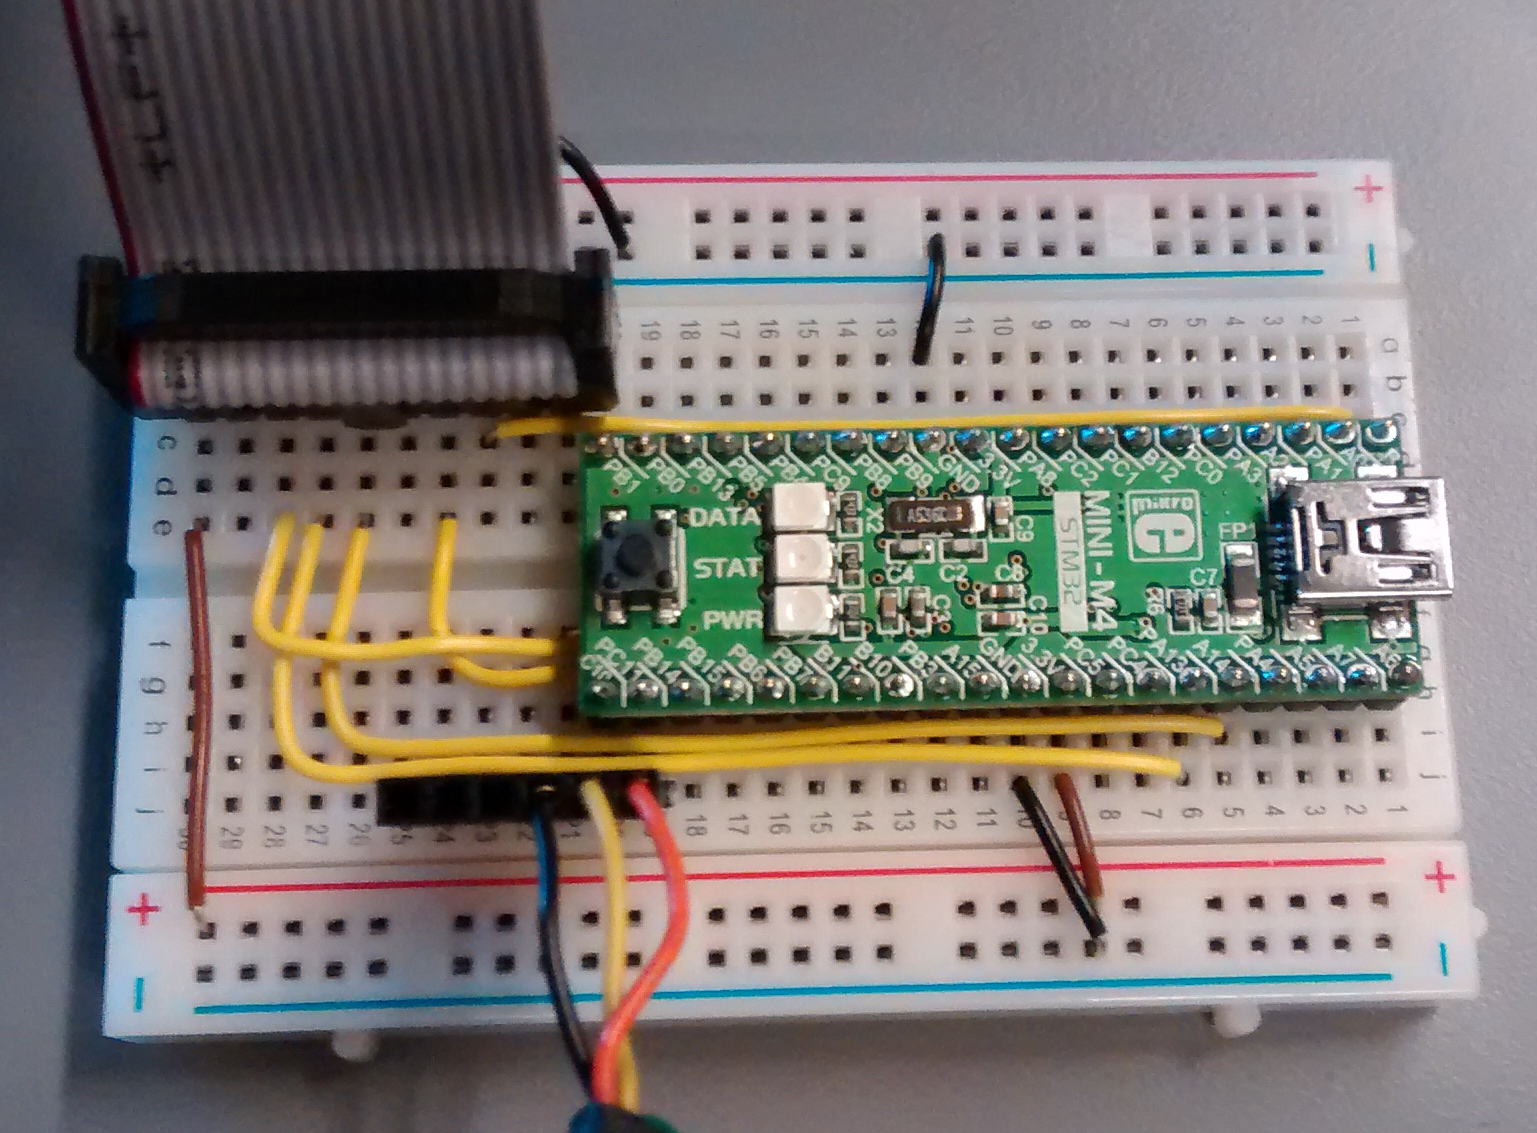
\includegraphics[width=.4\linewidth]{hardware/board_with_jtag_and_serial}
  \caption{Both the JTAG and serial interfaces}
  \label{fig:sub2}
\end{subfigure}
\caption{Connecting the board}
\label{fig:photo2}
\end{figure}

After this, the board is ready to be used in the development process.
The only drawback of this setup, is that it requires three USB ports:
one for power for the board, another one for the JTAG interface, and last
the serial communication. For detailed photos of the process, consult
Appendix \ref{app:hardware_setup}.

\subsection{JTAG Interface}
\label{ssec:JTAG_Interface}
Figure \ref{fig:sub1} represents the physical layout of the JTAG interface.
Since the JTAG connector has 20 pins, and only some of these are required
to communicate with the board, the set up process took some time to figure
out. The following diagram, shows the pinout of the JTAG and the 
corresponding pins on the microcontroller\textquotesingle s JTAG port.

\begin{figure}[H]
\centering
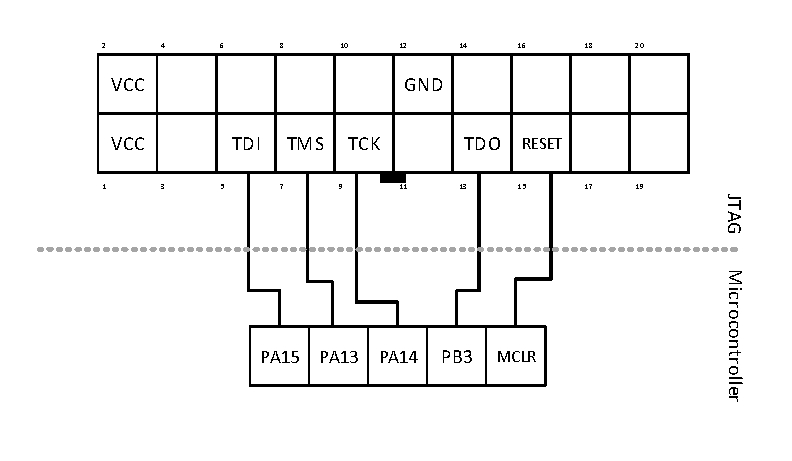
\includegraphics[width=\linewidth,keepaspectratio]{jtag_interface.pdf}
\caption{The connection of the JTAG interface}
\label{fig:jtag_interface}
\end{figure}

The tags on the upper part of figure \ref{fig:jtag_interface}, are
JTAG specific:
\begin{labeling}{RESET}
	\item [\textbf{TDI}]
		Test Data In pin
	\item [\textbf{TMS}]
		Test Mode State pin
	\item [\textbf{TCK}]
		Test Clock pin
	\item [\textbf{TDO}]
		Test Data Out pin
	\item [\textbf{RESET}]
		used for resetting the target device. This is connected to the 
		MCLR (Master Clear or Reset) pin of the board
\end{labeling}

The tags on the lower part of the figure represent the pins of the 
microcontroller, where $P$ stand for port, $A$ or $B$ for the port
identity ($PORTA$ or $PORTB$) and the number is the individual GPIO needed.

A driver \footnote{STSW-LINK009 v1.02} 
is needed to be installed on Windows machines, in order to
recognize and program using ST-LINK/v2.

\section{Source Structure}
The following sections describes different aspects the software used and
the source code located in the project root directory (ESS7\_project) denoted as `/'.
Below the root folder,
all the source code and compiled binaries are roughly structured as listed
in figure \ref{fig:source_structure}:

\begin{figure}[H]
	\dirtree{%
.1 /.
	.2 build.
		.3 ....
	.2 src.
		.3 drivers.
			.4 ....
		.3 kernel.
			.4 ....
		.3 partitions.
			.4 ....
			.4 utils.
	.2 third\_party.
		.3 ARINC.
			.4 APEX.
				.5 ....
		.3 CMSIS.
			.4 ....
		.3 linker\_scripts.
		.3 STM32F4xx\_HAL\_Driver.
			.4 ....
	.2 ....
	}
	\caption{A rough depiction of the source file structure.}
	\label{fig:source_structure}
\end{figure}


\section{Toolchain}
To write, compile and load code to the embedded platform,
a regular computer is used with ones editor of choice,
a C compiler and a programmer unit to transmit the code by the JTAG interface (\ref{ssec:JTAG_Interface}).
The toolchain is adopted from AAURacing\cite{aauracing} which uses a similar chip and develop on Linux\/OSX.
For this project the toolchain has been generalized to also work in windows 10 (later edition?).
In the rest of the section the toolchain and source code(one or two words?) structure is explained.

\subsection{CMAKE}
\label{ssec:cmake}
CMake is used to setup construct the makefiles for the project.
It's of little benefit comparing to write the makefiles from scratch,
but has been adopted in (this OS), since it came with the toolchain.

\begin{displayquote}
CMake is an open-source, cross-platform family of tools designed to build,
test and package software.
CMake is used to control the software compilation process
using simple platform and compiler independent configuration files,
and generate native makefiles and workspaces
that can be used in the compiler environment of your choice\cite{cmake}.
\end{displayquote}

Like Make, CMake is run from a file containing a set instructions on a project.
The instructions can be seperated in a nested structure of files to contain complexity (can you say that?).
A project can have multiple CMake files,
they all have to be named CMakeLists.txt and hence are placed in seperate folders.
The main CMake file is placed in the root-folder of the project and contains the main compiler information.
Specific information about compile targets and their files
are placed in sub files in folders as depicted in figure \ref{fig:cmake_files}.

\begin{figure}[H]
	\dirtree{%
.1 /.
	.2 src.
		.3 CMakeLists.txt.
	.2 third\_party.
		.3 CMakeLists.txt.
	.2 CMakeLists.txt.
	}
	\caption{Placement of CMakeLists.txt files in source directory.}
	\label{fig:cmake_files}
\end{figure}

As denoted by the first line of the CMakeLists.txt file in `/', no less than version 2.8.8 of CMake is required.
The rest of the file set up:

\begin{itemize}
	\item the compiler to use
	\item a list of compiler flags (section \ref{sssec:compiler_flags})
	\item commonly used include paths
	\item two required defines (section \ref{ssec:gcc})
	\item a command to flash the target device using OpenOCD (section \ref{ssec:openocd})
\end{itemize}

Using CMake followed by Make results in a tree of makefiles and objects,
which can be contained by running CMake and Make from within a build folder.
A complete tutorial on how to get started using the build system can be found in Appendix \ref{app:tutorial}.

Make is a UNIX tool\cite{gnu_make} often used to order many calls to GCC in C language projects.
Objects are compiled in separate calls to GCC and
Make provides features to set up a dependency tree of calls when many objects are linked together in a target.

\subsection{GCC}
\label{ssec:gcc}
The GNU Compiler Collection or GCC is used for compiling and linking the C files into a target called `OS'.
Compiling to the ARM architecture a cross compiled version of GCC is necessary,
in this case the arm-none-eabi-gcc compiler which is available in all never Ubuntu versions\cite{arm_gcc}.

\subsubsection{Compiler Flags}
\label{sssec:compiler_flags}
The compiler relies on a list of flags to compile the code to the programmers liking.
The sub section will cover the necessary or otherwise important flags for compiling the (OS).
The entries table \ref{tab:gcc_flags} can be found in the main CMakeLists.txt as referred to in section \ref{ssec:cmake}.

\begin{table}[H]
	\centering
	\begin{tabular}{|c|p{10cm}|}
		\multicolumn{2}{c}{\textbf{MCU flags}} \\
		\multicolumn{2}{c}{These options can be found at gcc.gnu.org \cite{gcc_arm_options}.} \\
		\hline
		-mcpu=cortex-m4   &
		This specifies the name of the target ARM processor. \\
		\hline
		-mtune=cortex-m4  &
		This option specifies the name of the target ARM processor for which GCC should tune the performance of the code. \\
		\hline
		-mthumb           &
		Generate code that executes in Thumb state. \\
		\hline
		-mlittle-endian   &
		Generate code for a processor running in little-endian mode. \\
		\hline
		-mfpu=fpv4-sp-d16 &
		This specifies what floating-point hardware is available on the target. \\
		\hline
		-mfloat-abi=hard  &
		Specifies which floating-point ABI to use.
		`hard' allows generation of FPU-specific floating-point instructions. \\
		\hline
		-mthumb-interwork &
		Generate code that supports calling between the ARM and Thumb instruction sets. \\
		
		\hline
		\multicolumn{2}{c}{} \\
		\multicolumn{2}{c}{\textbf{Linker flags}} \\
		\multicolumn{2}{c}{These options can be found at gcc.gnu.org \cite{gcc_linking_options}.} \\
		\hline
		-Wl, -T.../file.ld &
		Use the linker-script STM32F415RG\_FLASH.ld in the folder
		/third\_party/linker\_scipts (section \ref{ssec:linker_script}). \\
		\hline
		-nostartfiles   &
		Do not use the standard system startup files when linking.
		Used to force GCC to use a custom implementation of Newlibc implemented functions. \\
		\hline
		-Map=./result.map &
		Print a link map to the file result.map showing where object files and symbols are mapped into memory. \\
		
		\hline
		\multicolumn{2}{c}{} \\
		\multicolumn{2}{c}{\textbf{Debugging flags}} \\
		\multicolumn{2}{c}{These options can be found at gcc.gnu.org \cite{gcc_debug_options}.} \\
		\hline
		-g &
		Produce debugging information. \\
		\hline
		-ggdb &
		Produce debugging information for use by GDB. \\
		
		\hline
		\multicolumn{2}{c}{} \\
		\multicolumn{2}{c}{\textbf{C flags}} \\
		\multicolumn{2}{c}{These options can be found at gcc.gnu.org \cite{gcc_c_dialects}.} \\
		\hline
		-std=c99 &
		Determine the language standard to be ISO C99. \\
		\hline
		-fms-extensions &
		Accept some non-standard constructs, useful in some static structures (section ref). \\
		\hline
	\end{tabular}
	\caption{Showing the important GCC flags used to compile the OS.}
	\label{tab:gcc_flags}
\end{table}

There are two important flags, which haven't been mentioned in table \ref{tab:gcc_flags}.
the \texttt{-DHSE\_VALUE=16000000} and \texttt{-DSTM32F415xx} aren't compiler options but definitions passed to GCC to use at compile-time.

\texttt{-DHSE\_VALUE=16000000} defines the value of the external oscillator in hertz.
Specifically it defines \texttt{HSE\_VALUE} to be 16 million hertz as is specified in \cite{hse_value}.
The input of the external oscillator is used as the source for the main clock (some ref to clock setup?).

\texttt{-DSTM32F415xx} simply adds \texttt{STM32F415xx} as a definition at compile-time.
It's used by the HAL library to determine which processor to set up for.

\subsubsection{Linker Script}
\label{ssec:linker_script}
A linker script is used by the compiler to determine where to place different sections of the compiled binary.
Because of this, everything in the output binary gets an offset that matches the memory layout described in section \ref{sec:memory_map}.
The file \texttt{result.map} (table \ref{tab:gcc_flags}) can be used post compilation to determine the location of all symbols in the binary,
as a way to debug the linker-script.\\

The linker-file STM32F415RG\_FLASH.ld is part of the toolchain and is simple to edit to fit any member of the STM32F4 family.
In this project the only necessary change is the definition of flash to be 1MB of size.
Beyond that, the changes depends on the partition requirements on the system.\\

Listing \ref{linker_mem_overview} shows how the memory layout is defined in the linker script.
While \texttt{FLASH}, \texttt{RAM} and \texttt{CCMRAM} defines mappings of memory in hardware (see section \ref{sec:memory_map}),
\texttt{OS}, \texttt{DUMMY1}, \texttt{DUMMY2} and \texttt{STDIO\_SYS} defines the location and sizes of the system memory.
In listing \ref{linker_mem_overview}, \texttt{ORIGIN} denotes the starting address of a section of memory
and \texttt{LENGTH} denotes the size of the section.\\

\begin{minipage}{\linewidth}
\begin{lstlisting}[
	firstnumber=40,
	label=linker_mem_overview,
	caption=\textit{third\_party/linker\_scripts/STM32F415RG\_FLASH.ld}]
/* Specify the memory areas */
MEMORY
{
  FLASH (rx)     : ORIGIN = 0x08000000, LENGTH = 1024K
  OS (rx)        : ORIGIN = 0x08000000, LENGTH =   64K
  DUMMY1 (rx)    : ORIGIN = 0x08010000, LENGTH =    8K
  DUMMY2 (rx)    : ORIGIN = 0x08012000, LENGTH =    8K
  STDIO_SYS (rx) : ORIGIN = 0x08014000, LENGTH =    8K
  RAM (xrw)      : ORIGIN = 0x20000000, LENGTH =  128K
  CCMRAM (rw)    : ORIGIN = 0x10000000, LENGTH =   64K
}
\end{lstlisting}
\end{minipage}

By default all symbols and associated memory goes into the \texttt{OS},
Only when a partition is specifically defined to a location in the linker-script,
can it be separated from the OS.
Listing \ref{linker_example} shows how to allocate a specific partition.
The linker-script uses the fact that every partition is compiled as a library,
and the library name is added in the listed format under its corresponding label
(in this example: \texttt{STDIO\_SYS}).
This scheme insures the code is separated from the kernel in flash.
It does not, however, separate the statically allocated variables and structures in RAM.\\

\begin{minipage}{\linewidth}
\begin{lstlisting}[
	firstnumber=85,
	label=linker_example,
	caption=\textit{third\_party/linker\_scripts/STM32F415RG\_FLASH.ld}]
.stdio_sys :
{
  . = ALIGN(4);
  libstdio_sys.a:*
  . = ALIGN(4);
} >STDIO_SYS
\end{lstlisting}
\end{minipage}

Similar to listing \ref{linker_example},
the other partitions compiled libraries are confined to a space in flash,
as defined by their labels in \ref{linker_mem_overview}.

\subsection{OpenOCD}
\label{ssec:openocd}
Open On-Chip Debugger or OpenOCD \cite{openocd} is used together with the (hardware goes here) to program the chip and create a channel for GDB to debug the system on-chip.
The CMakeLists.txt file in project root defines a function running the following commands using OpenOCD:

\begin{itemize}
	\item \texttt{init} - Initialize connection
	\item \texttt{reset halt} - Reset and halt the system
	\item \texttt{flash write\_image erase \$\{elf\_file\}} - Write binary image to chip
	\item \texttt{reset run} - Reset chip and start normal execution
\end{itemize}

Above, \texttt{\$\{elf\_file\}} is the compiled output binary.

After execution of this command, OpenOCD will remain open and connected to the
chip and it will accept incoming connections on port 3333 for
GDB debugging as a GDB server (see more in \ref{ssec:gdb}.

\subsection{GDB}
\label{ssec:gdb}
\todo{Write GDB version}
The GNU Project debugger\cite{gdb}, GDB, is an open source software debugger
built to compliment the GNU Project compilers, GCC (see \ref{ssec:gcc}). It
allows programmers to more intelligently debug their applications.
GDB can\\
\begin{itemize}
	\item attach to a remote program, even running on a different piece of
	hardware. 
	\item pause execution of a program at specified lines of code with
	breakpoints.
	\item show the content of memory, either by direct a addressing or by
	variable name.
	\item if the hardware supports it, show the value of each CPU register.
	\item execute code line by line, letting the programmer see how each line
	affects the state of the program, and in case of crashing code, which line
	of code crashes the program.
\end{itemize}
This feature set, makes GDB especially useful for tracking down complex bugs and
bugs in otherwise inaccessible systems, e.g. systems with no screen to directly 
print to. GDB also allows programmers to investigate buggy code while it is
running, as opposed to after-the-fact debugging of logging, printing, etc.
Many advanced text editors and integrated development environments feature
direct seamless GDB integration. Outside of such programs, GDB can be run in 
command line.

To debug the code running on the chip, an active OpenOCD connection to the chip
is required. When OpenOCD is connected, it will act as a GDB server. GDB can
be connected to OpenOCD with the command \texttt{target remote localhost:3333}.

\section{Drivers}

Setting up the drivers took place in the early phases of the project. Their
functionality rely a lot on the HAL library. Even though the process is
quite straightforward, there is some learning involved in how to use the
HAL library. The library\textquotesingle s documentation is a good starting
point, and the things it lacks can be found in the 
microcontroller\textquotesingle s datasheet.

\subsection{System clock}
\label{ssec:system_clock}
The initial setting for the clock is that it uses the internal oscillator,
which runs at 16MHz. In order to get the maximum speed supported by the
CPU, the board needs to be configured to multiply this frequency.
However, instead of using the internal oscillator, which can be imprecise, 
the Mini-M4 
board has an external oscillator\footnote{Featuring less wander (slow
 variations due to temperature and aging) and jitter(fast variations)} 
that can be used as the main clock 
source. This is represented in figure \ref{fig:system_clock} with the HSE
tag. These tags refer to the location and the speed of the oscillators
present on the board or inside the microcontroller:

\begin{labeling}{HSE}
	\item[\textbf{HSE}]
		high-speed external oscillator, the main clock source
	\item[\textbf{HSI}]
		high-speed internal oscillator, not used
	\item[\textbf{LSE}]
		low-speed external oscillator, used by the real-time clock
	\item[\textbf{LSI}]
		low-speed internal oscillator, used by the independent watchdog
		timer
\end{labeling}

\begin{figure}[H]
\centering
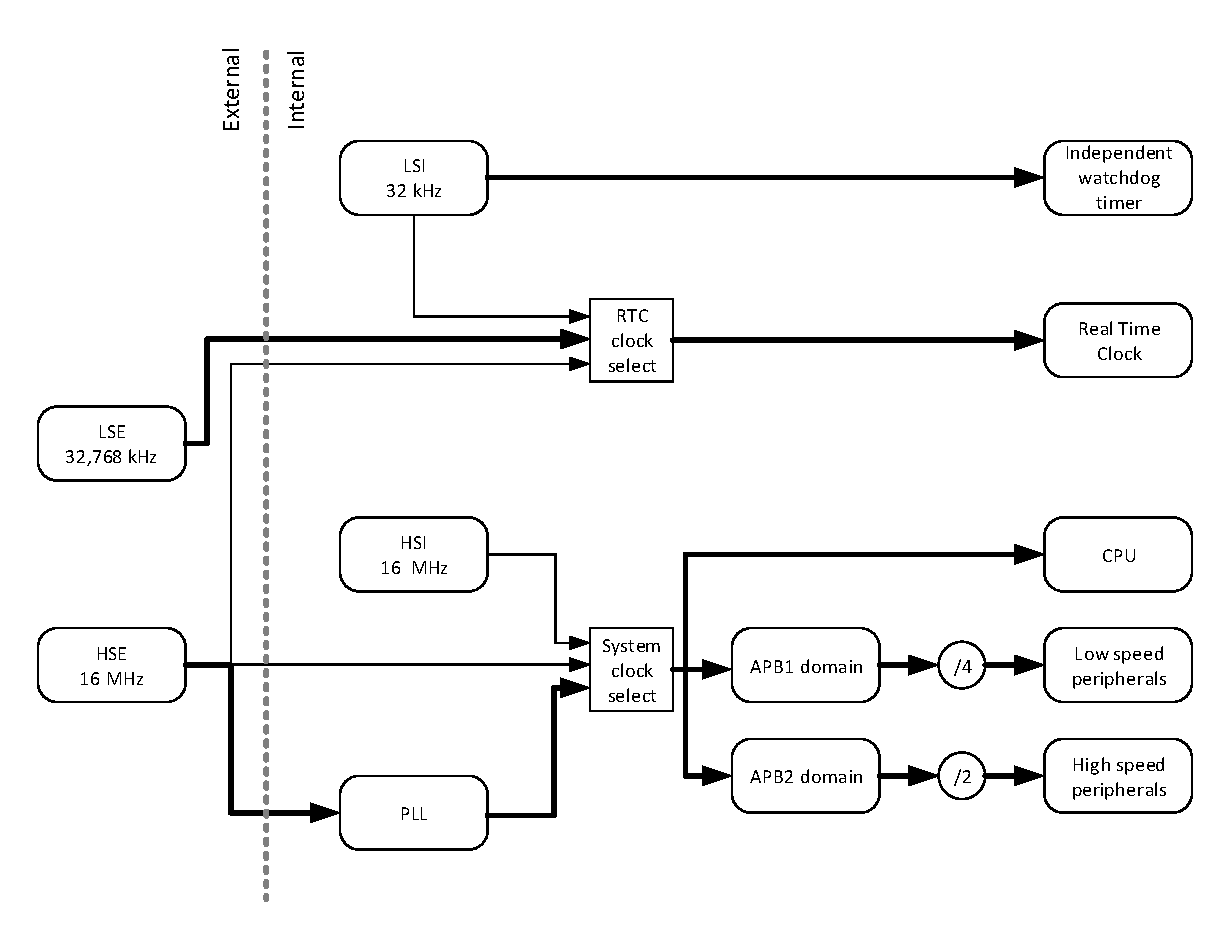
\includegraphics[width=\textwidth]{system_clock.pdf}
\caption{System clock overview \cite{reference_manual_216}}
\label{fig:system_clock}
\end{figure}

The lower part of figure \ref{fig:system_clock} shows that the frequency
of the HSE is multiplied by a PLL(Phase-locked loop) system, before it gets
to the clock selection block. This is the frequency supplied to
the CPU and memory through the AHB bus, and scaled down for the peripheral buses. These buses are divided into low and high speed domains as:

\begin{labeling}{APB1 domain}
	\item[\textbf{AHB}]
		Advanced High-speed bus. This runs at 168 MHz, and connects
		mainly the CPU, memory and the GPIOs.
	\item[\textbf{APB1 domain}]
		low-speed domain, running at 42 MHz. This includes among other 
		peripherals the UART.		
	\item[\textbf{APB2 domain}]
		high-speed domain, running at 84 MHz.
	\end{labeling}

The PLL registers\footnote{Specifically the division/multiplication 
factor registers} 
have to be set up in such a way that the frequency it 
generates is compatible with the prescaling settings of the peripheral
buses.

\subsection{UART}
The UART allows the transmission and reception of the information between the STM32 and the outside. The 
communication is made by one character at a time. The transmission is activated by the interrupts and it 
can happen both ways simultaneously, or one way at a time. An UART has a fractional baud rate generator 
system, yet it is limited by the GPIO frequency, which has 4 levels of frequency, input and output 
registers, transmit/receive control, read/write control logic, and transmit/receiver buffers. It is also 
possible to communicate with the UART using a screen, as an important output for debugging. The 
function used allows the transmission or reception of one character of a time, of the message sent by the 
\texttt{printf} function. The UART used was the UART4 of the STM32 connecting the wires to the PIN's 10 and 11.

\subsection{LEDs}
The LEDs are used mainly for debugging. There are three LEDs on the 
Mini-M4 board, two of them being programmable. Since they are connected
to two pins of a GPIO ports, these pins needs to be initialised first.
Afterwards, 
by using the functions defined in the HAL library, these pins can be 
turned high, low or toggled, thus changing the state of the LEDs.

\subsection{Delay}
\label{ssec:delay}
The delay function is also used for debugging, giving the developers the 
chance of seeing \textit{when things are happening}. This is because most of the
program instructions are executed so fast, that the they appear to be
instant to humans. 
Delay is defined in the HAL library, and relies on the SysTick.

SysTick is a timer\footnote{Fed with the system clock optionally 
divided by 8} that can 
be used to generate the main system event clock.
In fact, that is exactly how the HAL library has it implemented. Its
default time base is 1 millisecond. This means that every millisecond,
SysTick generates an interrupt to look after sensor values, scheduling or
basic timing tasks. To see a more detailed explanation of the SysTick
timer consult \ref{sssec:systick}.

\subsection{MPU}
As the regions are power of 2, as shown in the picture, the bigger partition is the more likely it 
is to have spare space, since it becomes harder to fit it completely in a region.\\
\begin{figure}[H]
\centering
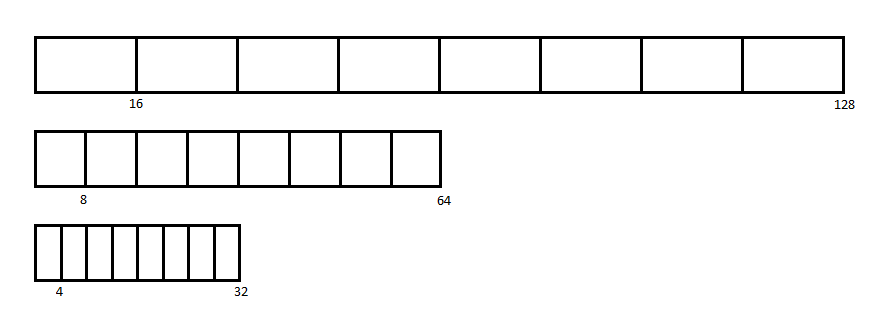
\includegraphics[width=15cm]{partitions/partitions2.png}
\captionof{figure}{Example of 3 memory region sizes}
 
\end{figure}
Lets take, as an example, 5 partitions with the sizes of 20, 65, 120, 80 and 40bits.\\
\begin{figure}[H]
\centering
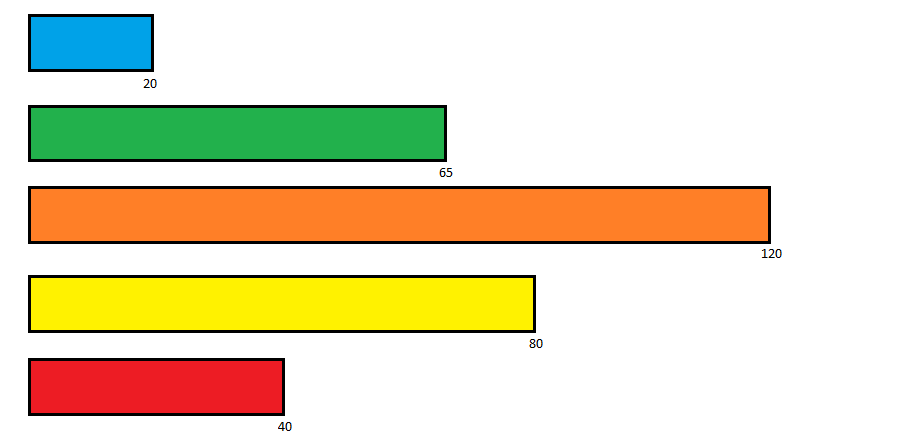
\includegraphics[width=15cm]{partitions/partitions1.png}
\captionof{figure}{Example of 5 partitions sizes}
 
\end{figure}
If they were just allocated in the most suited region for each, the memory needed would be of 480bits, 
leaving 155bits unused.\\
\begin{figure}[H]
\centering
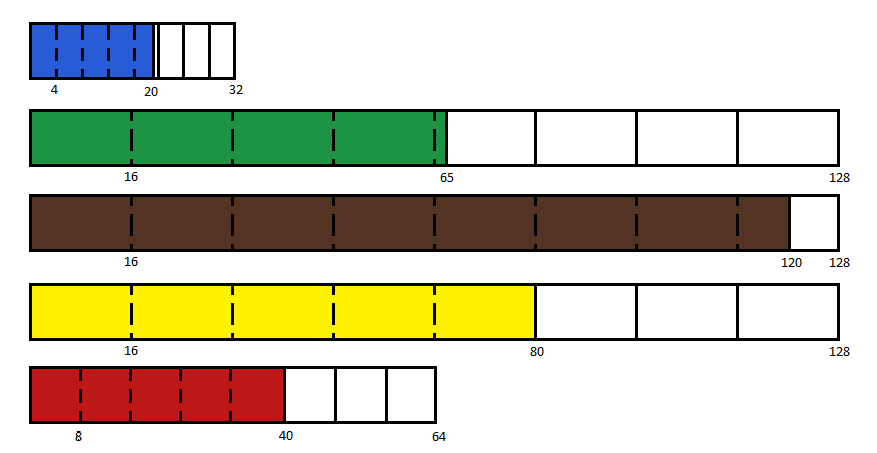
\includegraphics[width=15cm]{partitions/partitions3.png}
\captionof{figure}{Partition memory distribution in different regions}
 
\end{figure}
The first allocate are the biggest partitions and if there are empty subregions, the system tries to 
allocate smaller partitions in those gaps, like shown in the figure, using only 384bits.\\
\begin{figure}[H]
\centering
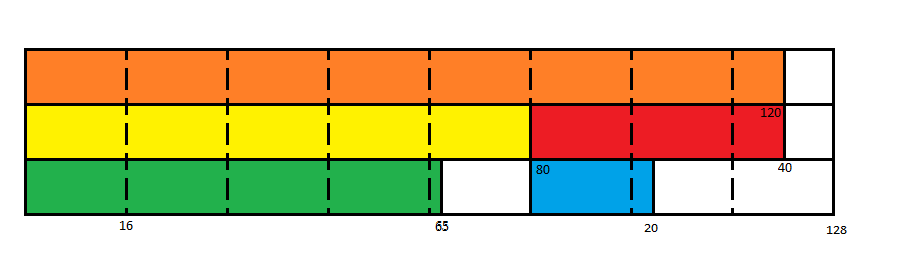
\includegraphics[width=15cm]{partitions/partitions4.png}
\captionof{figure}{Partition memory distribution in the same regions}
 
\end{figure}
In case that a certain partition doesn't full fill the subregion, their size gets updated with the full 
remaining subregion area, 
instead of leaving those parts always empty. That can also help to avoid some errors, for example if the 
initial defined size wasn't enough for the different processes allocated by that partition.\\
\begin{figure}[H]
\centering
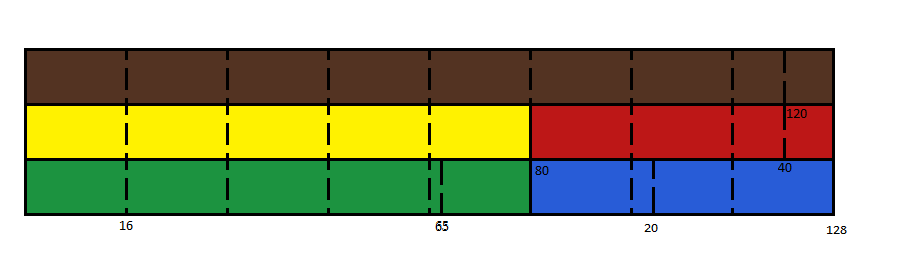
\includegraphics[width=15cm]{partitions/partitions5.png}
\captionof{figure}{Memory extension of the partitions sizes}
 
\end{figure}

\subsection{Timing}
\label{ssec:timing}
This driver is used for accurately measuring the execution time of different
functions. It uses the DWT (Data Watchpoint and Trace support)
internal peripheral registers defined in the ARM-M4 Architecture 
manual \cite{arm_architecture}.
Since the HAL library does not define them, there is need to access them
by their addresses. Their address range can be seen in the upper part of
figure \ref{fig:memory_model}, while the register used by this driver are 
shown in listing \ref{list:time_get}.

\begin{minipage}{\linewidth}
\begin{lstlisting}[
	firstnumber=9,
	label=list:time_get,
	caption=\textit{src/drivers/time\_get.c}]
volatile unsigned int *DWT_CYCCNT  = (unsigned int *)0xE0001004;
volatile unsigned int *DWT_CONTROL = (unsigned int *)0xE0001000;
volatile unsigned int *SCB_DEMCR   = (unsigned int *)0xE000EDFC;
\end{lstlisting}
\end{minipage}

\textit{DWT\_CYCCNT} is a 32 bit counter, that when enabled counts
the number of core cycles. \textit{DWT\_CONTROL}\footnote{Referred to
as DWT\_CTRL in the ARM documentation} is the control register for the
Data Watchpoint and Trace support. By setting its least significant bit,
the cycle counter mentioned above is enabled. The last register,
\textit{SCB\_DEMCR} has to do with Debug Exception and Monitor Control Register,
and is used to manage exception behaviour under debug.

At a core frequency of 168 MHz, \textit{DWT\_CYCCNT} would be
incremented every 5.45 nanoseconds. In order to convert the number 
of cycles into time, the function in listing \ref{list:time_convert}
was used.

\begin{minipage}{\linewidth}
\begin{lstlisting}[
	firstnumber=33,
	label=list:time_convert,
	caption=\textit{src/drivers/time\_get.c}]
int64_t convert_cycles_to_time(uint32_t cycles)
{
    return (int64_t)((cycles / 168) * 1000);
}
\end{lstlisting}
\end{minipage}

The returned value is a 64 bit signed integer, as the \arinc{} standard 
specifies \cite{arinc_time}. the only problem with this, is that while 
the count is done in the range of nanoseconds, the sampling frequency
gives a 5.45 nanosecond step. In order to fully comply with the standard,
we would need a timer running at at least 1 GHz\footnote{Produces 1
 nanosecond steps}.

\subsection{Watchdog timer}
% \ http://electronics.stackexchange.com/questions/123080/independent-watchdog-iwdg-or-window-watchdog-wwdg
The microcontroller has two watchdog timers ready to reset the program, in case of an error.
The first one, the independent watchdog timer is based on an oscillator
\footnote{LSI running at 32 kHz, seen in the upper part of
 \ref{fig:system_clock}}
that can only be used by it.
\todo{focuses on hardware fails} This way,
the the watchdog could catch a fault in the program, even if the other
oscillators fail. Its basic functionality is represented in figure
\ref{fig:watchdog}. After the program starts running, a function is called
that initialises and starts the watchdog timer. Here, a period of time is defined, in which the program has to refresh (reload) the watchdog timer.
If this fails to happen, either by mistake, the developer forgetting to 
call the refresh function, or by a software/hardware fault, the watchdog 
timer restarts the program (depicted with the red arrow).

\begin{figure}[H]
\centering
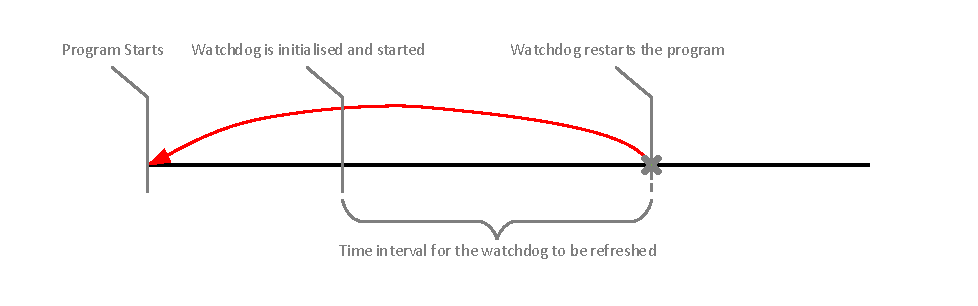
\includegraphics[width=\linewidth,keepaspectratio]{watchdog.pdf}
\captionof{figure}{Basic watchdog timer functionality}
\label{fig:watchdog}
\end{figure}


The second watchdog timer, is called a window watchdog.
\todo{focuses on software fails} In contrast 
to the independent watchdog, one can provide a time interval in which
the timer has to be reset. Resetting the timer outside this interval
(as well as not resetting it in the mentioned time window) would restart
the program. It uses the system clock, which means that if this fails,
the watchdog won\textquotesingle t be able to reset the system. this 
watchdog has not been implemented, but its functionality is relevant 
to \OSname{}.

In regards to what the standard specifies, that the processor should be able
to isolate a partition that fails \cite{arinc_page_12}. This could be done by 
using the window watchdog timer to define the time intervals for partitions 
to run. The feature called Early Wakeup Interrupt can be used to do some
safety operations, just before the reset is done by the watchdog.
\cite{reference_manual_716}.
In short, if the window watchdog is not reset in the window interval it
receives (correspondent to each partition), then the EWI will isolate the
partition and the microcontroller will be reset to continue its operation
with the remaining partitions.

\subsection{RTC}
The real-time clock was implemented as a way to give the system the
possibility to keep track of time. It was realised at a later point
that \arinc{} specifies that time keeping should be done in nanoseconds,
a range that the RTC is not capable of. This was the reason for continuing 
researching other ways of timing the system, as seen in:
\ref{ssec:timing}.

Anyway, the RTC could be used for timestamps on error logs and such,
as the standard specifies \cite{arinc_page_26}. The use of the LSE oscillator,
as well as the design of the RTC 
\footnote{Which includes all time components, as well as
subseconds and year correction}, make this a reliable
secondary clock source.

\section{XML configuration file}

Writing the XML configuration file was an evolutionary process throughout the implementation phase. To begin with, the example XML provided by the ARINC 653 standard was used. As functionality within the system became available, the example XML values were modified for the desired purposes. All content in the XML was written by hand, there is no tool support to modify the content.

\section{XML Parser}

The configuration of the OS is not usable in its XML format. \OSname\ is written in C; therefore a dynamic parser written in Python called createCStructs.py has been created to translate the XML and generate C structs.
\todo{reference for xmltodict}
Using an external library xmltodict.py, the XML is converted into a JSON structure which makes navigating and accessing sub nodes very easy as it becomes a nested dictionary structure containing lists.
The generation of the of the structs are handled as two separate files; xml\_data.h and xml\_data.c. 

\subsection{xml\_data.h}

xml\_data.h contains the static declarations for the structs written to the xml\_data.c, and the symbols for the xml\_data.c functions and variables. 
\\
The declarations for the structs are included into xml\_data.h from a file called type.h. The symbols for the functions and variables are written to the file whilst parsing the XML.

\subsection{xml\_data.c}

xml\_data.c is mostly dynamic and generated from the elements in the XML. 
The static elements of its generation are handled by two functions and the self.idle\_partition set in the init. The static functions are called write\_file\_c\_header and write\_file\_c\_footer. These functions write the static code needed at the beginning and end of the xml\_data.c file to function such as the includes and the endif.
The idle partition is not included in the XML. It is hard-coded into the partition loop as it is always required to exist. For more info about the idle partition refer to (chapter \ref{ssec:idle_part}) 
\\\\
There are four dynamic elements (partitions, partition\_memory, module\_schedule and connection\_table) which are acquired from the JSON structure. They and are looped through, populating formatted strings, and are then written to xml\_data.c.

\section{C Structures}

The data structure undergoes change during the translation from XML described in
section \ref{sec:design_schema} to C structs to support ease of use. The
structure of the data and relationships of the elements are presented in the
figure below.

\begin{figure}[H]	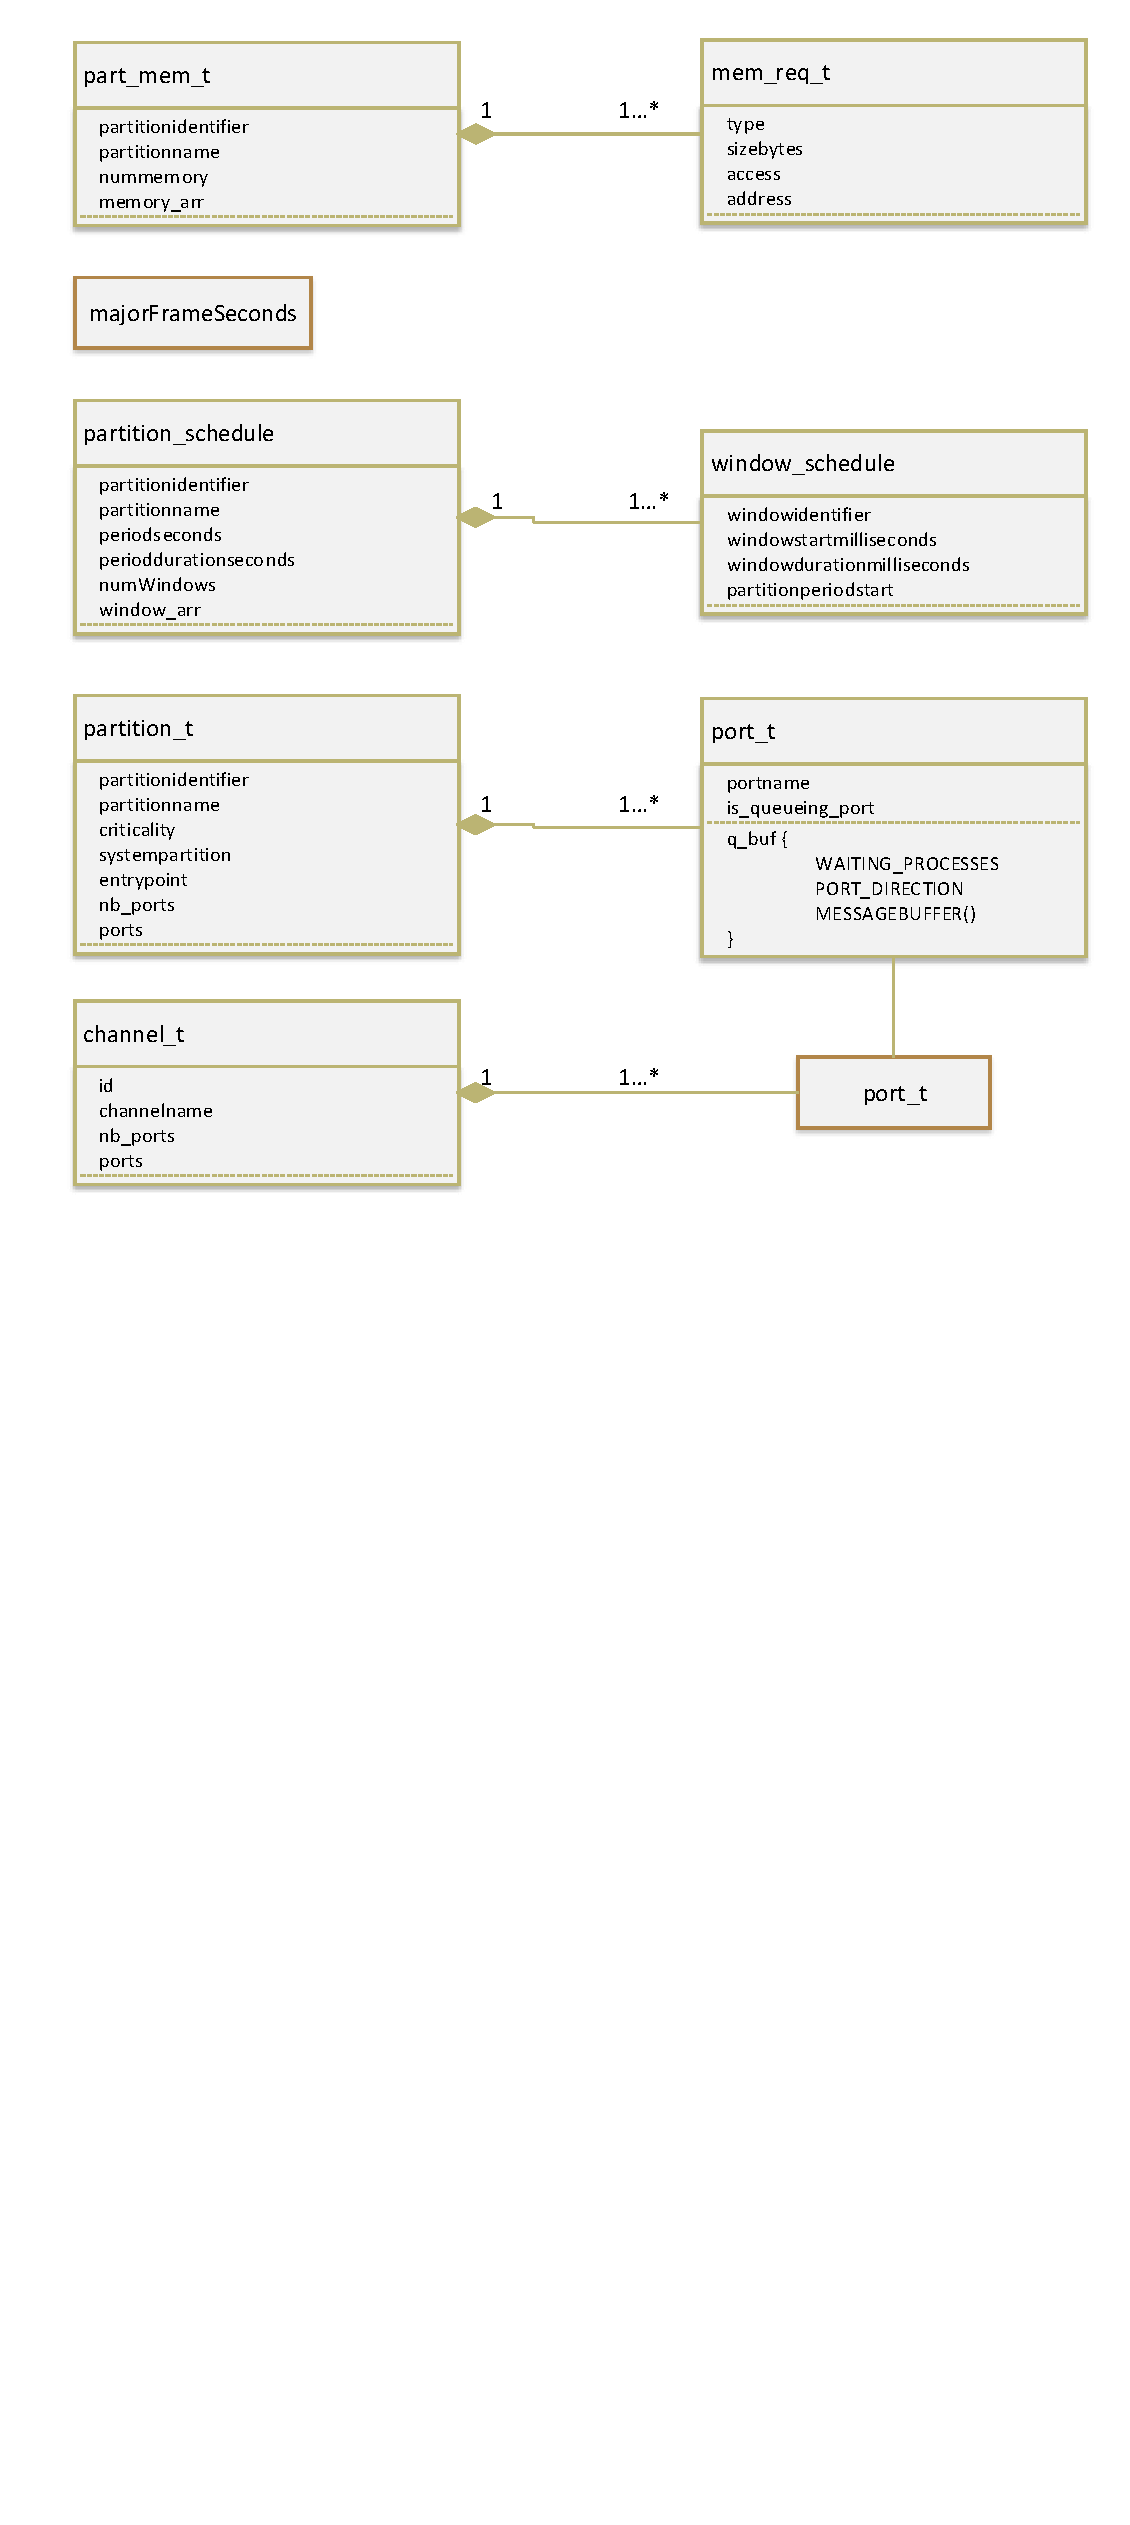
\includegraphics[clip=true,trim=0cm 20cm 0cm 0cm,width=\linewidth,keepaspectratio]{figures/cstructs.pdf}
	\caption{C structs design and relationships}
	\label{fig:cstructs}
\end{figure}

The global structure of ARINC\_653\_Module has been removed, its sub elements now exist without a dependency. 
Module\_schedule as also been removed, leaving its attribute majorFrameSeconds as an independent variable definition. 
partition\_memory (part\_mem\_t) and partition\_schedule have maintained their one to many structures with their sub elements. 
Partitions sub elements, sampling and queuing ports, have combined into a single structure called ports. 
The XML element Connection\_Table has been removed, and StandardPartition has
been transformed into a port reference list which shares an association with the ports.
\\\\
The following structures have been extended to contain an array of its substructures:
\begin{itemize}
	\item part\_mem\_t contains an array memory\_arr which references to the memory information of a given partition.
	\item partition\_schedule contains an array windows\_arr which references to the timing window in which a partition is executed.
	\item partitions\_t contains an array ports which references to the ports available to the partition.
	\item and channel\_t contains an array ports which references to the ports available to the partition.
\end{itemize}

each with an associated variable to indicate the number of elements in the array.\\

port\_t is a generic structure to define a port independent on its type as
detailed in section \ref{impl:ports}.

\section{OS kernel}
This section gives an overview of the the features in \OSname\ and how they are
implemented. At the end a feature list is provided to give summery of the features
and services implemented in \OSname .

\subsection{OS Initialization}
\OSname\ is initialized from the \texttt{main()} function in /src/kernel/main.c.
Its job is to set up the following:

\begin{enumerate}
	\item The main clock
	\item UART and clear the terminal
	\item Red and yellow LED
	\item The ports
	\item Partitions and their processes
	\item Construct a partition schedule
	\item Enter unprivileged mode by setting a bit in a register
\end{enumerate}

A more complete implementation of ARINC 653 would also have to setup the MPU.
Though the MPU is designed and testable code does exist, it is at this point yet
to be included into the kernel as a service and for this reason no setup is done.\\

The setup of the UART is fixed to use port C pin 10 and 11 with a baud-rate of
115200 baud. Setting it up is a matter of passing these arguments to the HAL
library and is not covered further in the report.\\
The same argument can be made about the LEDs which also not will be described.\\

The last action taken by the main function is enabling the SysTick interrupt and
entering unprivileged mode start the scheduler.\\

In the following the sections the main clock setup (section \ref{impl:clock_setup},
the partition and process setup (section \ref{impl:part_proc_setup}), and
partition schedule setup (section \ref{sssec:build_schedule}) is explained in
further detail.


\subsubsection{Main Clock Setup}
\label{impl:clock_setup}
The system clock is setup using its specific driver, explained in
\ref{ssec:system_clock}. The driver sets the core to run at 168 MHz, as
well as prescaling this frequency for the peripheral buses.


\subsubsection{Partition and Process Setup}
\label{impl:part_proc_setup}
The idle partition (explained in section \ref{sssec:schedule_building}) is set up
first using its entrypoint \texttt{idle\_main}.\\

The rest of the partitions listed in the auto-generated C file are initialised
by setting the number of active processes to one, setting up their specified
entrypoint with a memory address within their memory space and setting the rest
of the empty process entries to \texttt{DORMANT}.\\

Note that in this implementation every process is given 1KB of RAM to use for
stack. This can course a fault if partitions initializes more processes than
their defined memory spaces holds.


\subsubsection{Building the schedule}
\label{sssec:schedule_building}
The partition schedule is defined in the XML schema file as windows (see 
\ref{sssec:impl_windows}). Windows in the XML schema, as well as in xml\_data.c
file output by the schema parser, are ordered by partition, not chronologically.
Additionally, windows in the XML schema are not subelements of partitions, but
are instead separate elements, referencing the partition they belong to by ID.

As a result, to do any scheduling of windows, it is necessary to search through
all windows to find the next one within a major frame, and then search through
all partitions to find the partition with the same ID. To make matters more
complicated, the XML schema may contain implicit idle periods (periods with no
defined windows). To lighten the burden on the scheduler, the work to build a
schedule by ordering the windows chronologically and inserting explicit idle
periods are done during system initialisation.\\

Provided the same XML schema, the schedule is also always the same; each time
the system boots, a schedule identical to the one last used will be built.
In future builds of \OSname , the schedule should ideally be built by the XML
schema parser, to avoid rebuilding the same schedule during each boot of the
system.

The algorithm to build the schedule is as follows:\\
\begin{algorithm}[H]
\tcc{excluding implicit idle periods}
$totalWindows \leftarrow$ number of windows in xml\;
$desiredStartTime \leftarrow 0$\;
\tcc{This is just an arbitrary high number}
$earliestNextStartTime \leftarrow 5000$\;
$matchingWindow \leftarrow NULL$\;
\While{windows in schedule < $totalWindows$}{
	\ForEach{window $w$ in xml schema}{
		\If{start time of $w$ = $desiredStartTime$} {
			$matchingWindow \leftarrow w$\;
			break\;
		}
		\ElseIf{start time of $w$ > desiredStartTime and earlier than $earliestNextStartTime$}{
			$earliestNextStartTime \leftarrow$ start time of $w$\;
		}
	}
	\If{matching window is found}{
		$partition$\;
		\ForEach{partition $p$}{
			\If{ID of $p$ = ID of partition of $matchingWindow$}{
				$partition \leftarrow p$\;
				break\;
			}
		}
		insert window for $partition$ into schedule\;
		$desiredStartTime \leftarrow$ start time of $w$\;
	}
	\Else{
		insert window starting at $desiredStartTime$ and lasting
		$earliestNextStartTime - desiredStartTime$ for idle partition into schedule\;
		\tcc{This is just an arbitrary high number}
		$earliestNextStartTime \leftarrow 5000$\;
		$totalWindows++$\;
	}
}
\end{algorithm}

Provided that the data in the XML schema is valid, i.e. there is window 
referencing a partition that does not exist, and provided that the major frame
is shorter than 5000 (this number is easily changeable) time units, this
algorithm will create a schedule of chronologically ordered windows, including
windows pointing to the idle partition.\\

\begin{figure}
	\centerline{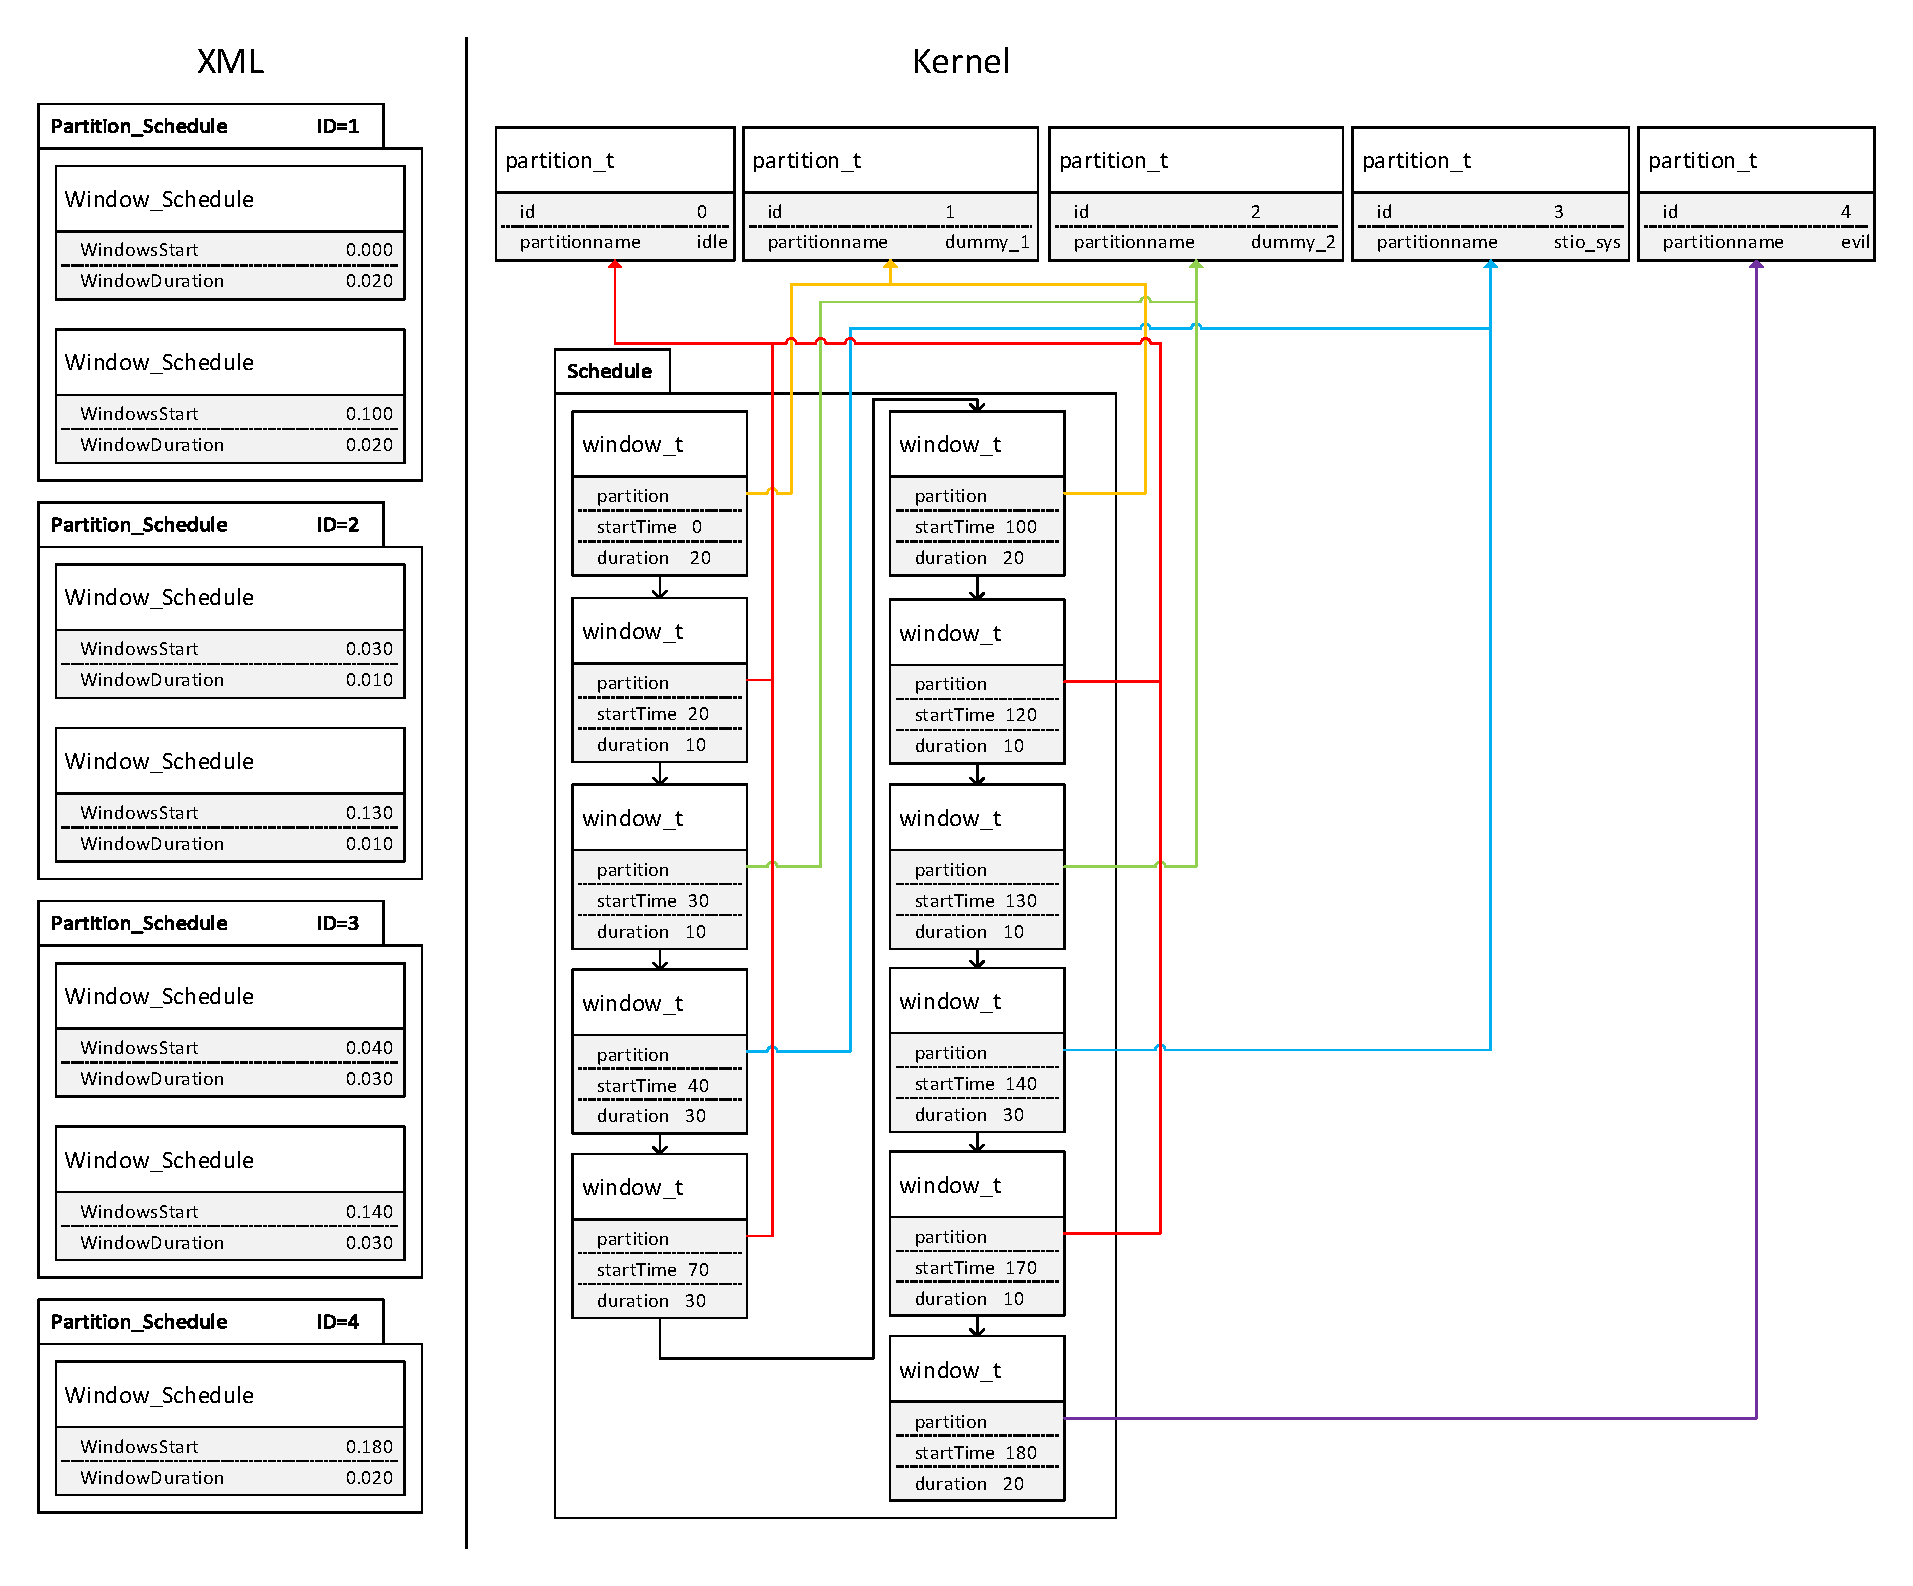
\includegraphics[width=\paperwidth,angle=90,clip,trim=0 1cm 0 0]{figures/demo_windows.pdf}}
	\caption{Windows as represented in the XML schema, and in the kernel after 
	the schedule has been build}
	\label{fig:demo_windows}
\end{figure}
Figure \ref{fig:demo_windows} shows what the finished schedule may look like,
given a certain schedule in the XML schema.


\subsection{Scheduling}
The ARINC 653 specification defines two levels of schedulers and the rules by
which these schedulers decide which processes may execute at any given time.
There are two different kinds of rescheduling, temporal rescheduling and event
driven rescheduling. Partitions are exclusively rescheduled because of time,
whereas processes may be rescheduled because of both time and events.
As for temporal scheduling, the ARINC 653 specification does not explicitly
specify a minimum or maximum time resolution for scheduling, though it does
imply a resolution of 1 nanosecond should be available\cite{arinc_time}.

For \OSname\ the SysTick is used for triggering temporal scheduling. This choice
also led to the choice of a time resolution of 1 millisecond. Scheduling is
never disabled; every millisecond the scheduler will be invoked and check which
process of which partition should run next. Therefore, increasing the resolution
of time, e.g. to 1 nanosecond, would increase the overhead of scheduling; the OS
would spend a greater amount of time handling scheduling compared to executing
user code.

Oppositely, decreasing the resolution would limit the places where \OSname\ is
viable, as certain tasks require a certain minimum resolution. For example,
assuming the system is continuously moving, a sorting robot has only a certain
time to identify objects before they pass by its sensors. If time resolution of
the underlying operating system of such a robot is too low, object may pass the
robots sensors before the code checking the sensors are rescheduled.\\

Though the \arinc\ specification implies a 1 nanosecond resolution, at least for
timed waits, this is not supported in \OSname . Given the maximum frequency of
168 MHz for the MINI-M4, a nanosecond resolution would be physically impossible.\\

Scheduling is triggered within the function \texttt{SysTick\_Handler}. This
function is called directly by the NVIC when the SysTick timer triggers an
interrupt. \texttt{SysTick\_} \texttt{Handler} function first saves the current
context, then invokes the partition scheduler, followed by the process scheduler.
Once the process scheduler finishes, the \texttt{SysTick\_}\texttt{Handler}
restores the context of chosen process and returns control to the NVIC.

\subsubsection{SysTick}
\label{sssec:systick}
The SysTick timer is a 24-bit decreasing timer that wraps when reaching zero.
Unlike other timers on the MINI-M4, this timer is specified as part ARMv7M
specification. Other timers are implementation specific; the vendor decides
which timers to add to a chip. Therefore, between two different boards, there
may be a different number of timers, and timers may have a different resolution.
This makes it more difficult to port code from one board to another. The SysTick
timer however, is guaranteed to be 24-bit on any board that implements it. In the
Cortex-M group of ARM microcontrollers, the SysTick timer is required for M3, M4
and M7; any code written for these can assume portability.\\

The clock source for the SysTick timer is the CPU clock, optionally divided by
eight. The reset value of the SysTick timer is programmable. This makes it
possible for software to program how often this timer wraps.
Unless otherwise specified, this timer operates in polling mode; software has to
poll for wraps, but it is possible to program the SysTick timer to trigger an
interrupt upon wrapping.

By default the HAL library sets up the SysTick timer to wrap every 1 millisecond
and to trigger an interrupt upon wrapping.

\subsubsection{Context Switching}
There are multiple different states the processor can be in, when a context
switch from one process to another occurs. The state indicates whether the
Master Stack Pointer or the Process Stack Pointer was used by the process,
and whether the FPU was used by the process or not. Because of this, the context
switch algorithm must start by determining the processor state in order to know
which registers
to save and which stack to save them to.\\
The processor state is saved in the LR register, and it can be one of
the possible six EXC\_RETURN values (see figure \ref{tab:exc-return}).\\
If the pre-empted process used the FPU, the FPU registers S16 to S31
should also be saved by software in addition to the general purpose registers.
Because of time constraint, this was not implemented.\\
The registers are saved entirely on the stack. Therefore, it is important for
the software to know which
stack pointer to use when saving the remaining registers. Therefore the first
thing the interrupt service routine (ISR) used for scheduling must do, is to inspect
the \excreturn\ value in the LR register to determine whether to use the
Master Stack Pointer or the Process Stack Pointer. The software must then, at
the address denoted by the stack pointer, save the registers that have yet to be
saved, and update the stack pointer, before saving both the stack pointer and
the \excreturn\ value to the process structure elsewhere in memory. This is all
done in assembly to make sure that there is complete control over which
registers are used, so as to avoid overwriting any registers that have yet to be
saved. This is absolutely necessary, as otherwise the state of register for a
process might be corrupted during a context switch. Additionally, any ISR used
for scheduling must be declared as naked\footnote{A naked function has no
compiler generated prologue and epilogue. This means that the compiler does not
save any registers on the stack before using them, and it does not restore them
before ending a function.}, to avoid the compiler changing registers before the
context can be saved, and to give complete control over which value is pushed to
the PC register at the end of the ISR. Listing \ref{list:context_save} show the
code that saves contexts on the stack.\\
\begin{figure}
\lstset{
	language=C,
	basicstyle=\footnotesize,
	showspaces=false,
	showtabs=false,
	showstringspaces=false,
	tabsize=4,
	breaklines=true
}
	\begin{lstlisting}[
		firstnumber=37,
		label=list:context_save,
		caption=\textit{src/kernel/context.h}
		]
__attribute__((always_inline))
static inline uint32_t context_save()
{
	// Create a new variable to store the context-saved-stack pointer of the previous process.
    // We explicitly choose the register to avoid GCC picking a register that hasn't been saved yet.
	register uint32_t stackpointer __asm("r0");
	// Context switch logic.
    // We only save R4-R11 on the stack, because the NVIC already saved the other registers before calling this function.
    __asm volatile (
        "AND	R1, LR, #0x0D	\n\t"		// Logical AND with 0xD
        "CMP    R1, #0x0D		\n\t"		// Use CMP to set EQ/NE flag
        "BEQ    use_psp			\n\t"		// Branch to use_psp if EQ is set
        "BNE    use_msp		 	\n\n"		// Branch to use_msp  if NE is set
        "use_psp:				\n\t"
        "MRS    %0, PSP			\n\t"		// Move Process Stack Pointer to R1 (the stackpointer variable)
        "STMFD  %0!, {R4-R11}   \n\t"		// Store registers R4 to R11 on the stack. (The FD in STMFB means fully descending [stack])
        "MSR    PSP, %0         \n\t"		// Update the actual PSP stackpointer register with the new value after STMFD.
        "B      exit			\n\n"		// Skip over the use_msp routine
        "use_msp:				\n\t"
        "MRS    %0, MSP			\n\t"		// Move Master Stack Pointer to R1 (the stackpointer variable)
        "STMFD  %0!, {R4-R11}   \n\t"		// Store registers R4 to R11 on the stack.
        "MSR    MSP, %0         \n\n"		// Update the actual MSP stackpointer register with the new value after STMFD.
        "exit:                  \n\t"
        : "=r" (stackpointer)
        : :
    );
    return stackpointer;
}
	\end{lstlisting}
\end{figure}

After the context has been saved, control is handed over to the scheduler, which
then decides which process should run next.\\
Once all the operations the ISR has completed, the context of the process
selected by the scheduler must be restored. From this point, the code is once
again written in assembly to avoid overwriting a register after it has been
restored. First, the registers saved by software on the stack must be restored,
then based on the \excreturn\ value that the process interrupted with, it can be
determined to which stack pointer register the new stack pointer must be pushed
to. Lastly, execution must return to the process by pushing the \excreturn\ value
to the PC register. The \excreturn\ value pushed to the PC register must be the
same as that read from the LR register when the process was interrupted.
Figure \ref{fig:scheduling_sequence_diagram} shows the flow when switching contexts.
Listing \ref{list:context_restore} show the source code that restores the
context of a process and branches to the \excreturn .
\begin{figure}[H]
	\centerline{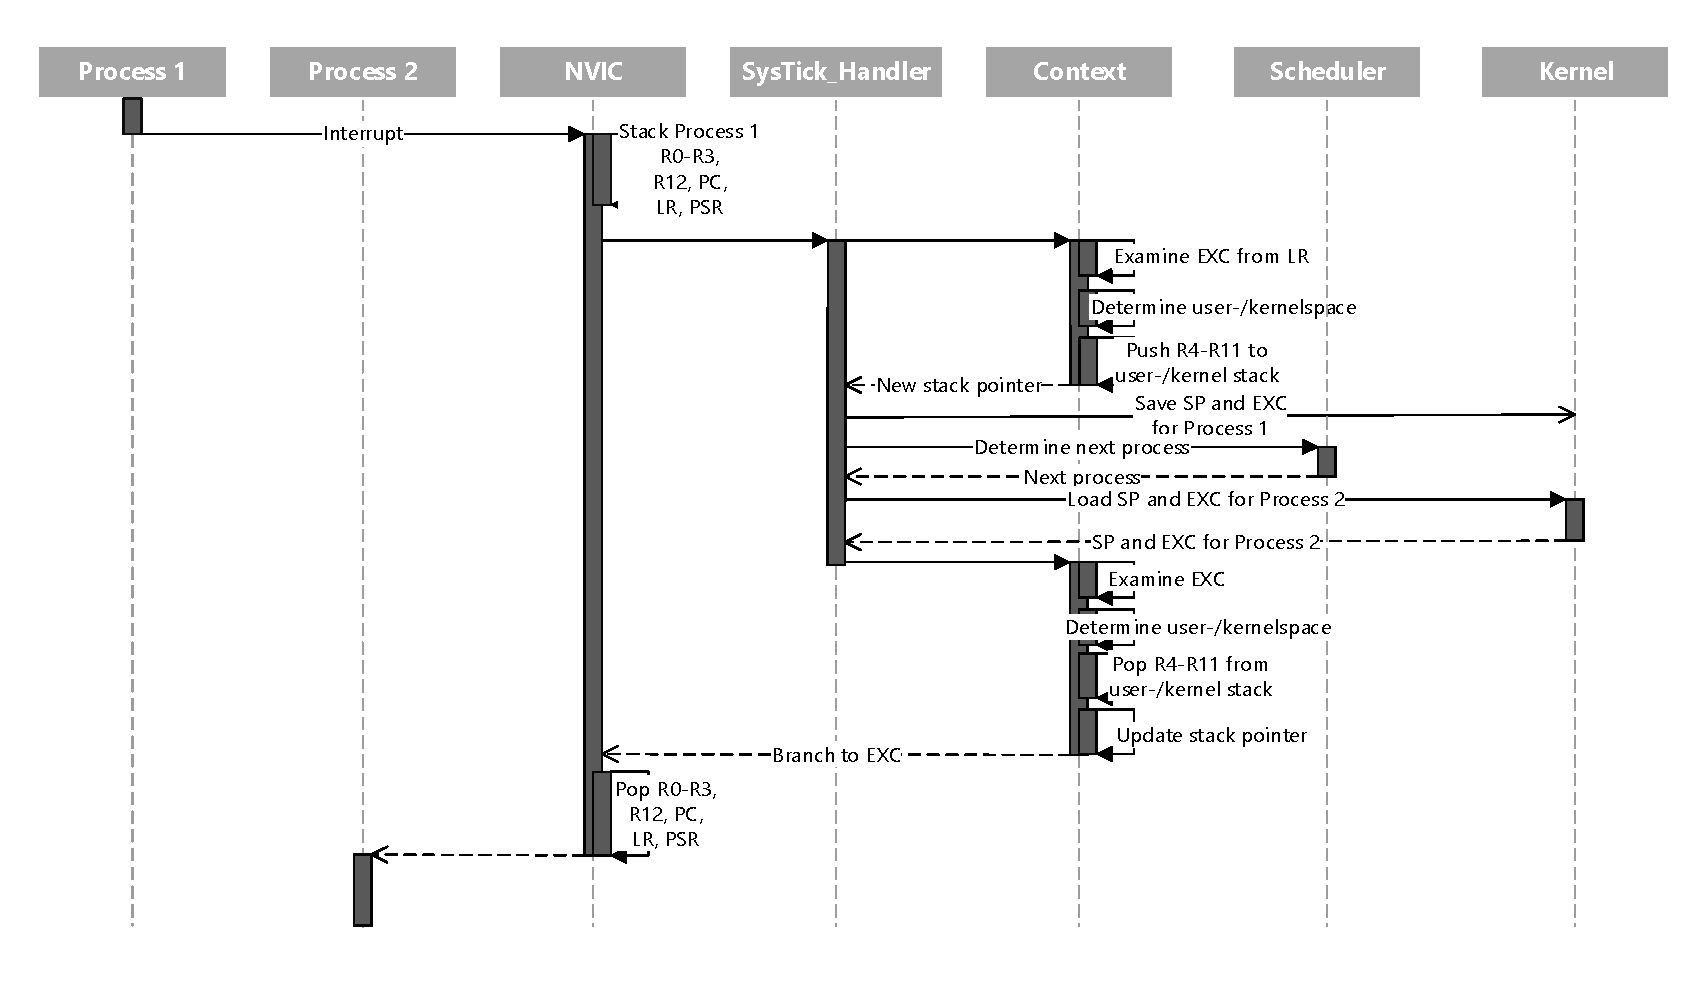
\includegraphics[width=\paperwidth-2cm,]{figures/scheduling_sequence_diagram.pdf}}
    \caption{This figure shows the steps involved in switching context from one
	process to another}
    \label{fig:scheduling_sequence_diagram}
\end{figure}
\begin{figure}[H]
\lstset{
	language=C,
	basicstyle=\footnotesize,
	showspaces=false,
	showtabs=false,
	showstringspaces=false,
	tabsize=4,
	breaklines=true
}
\begin{lstlisting}[
	firstnumber=66,
	label=list:context_restore,
	caption=\textit{src/kernel/context.h}
]
__attribute__((always_inline))
static inline void context_restoreAndSwitch(uint32_t stackpointer, uint8_t exc_return_value)
{
    // Restore the software context of the new process.
    // Variable data is loaded into static registers in the beginnning
    // to make sure the GCC doesn't decide to use the registers R4-R11 after
    // they've been restored; that would be catastrophic!
    __asm volatile (
        "MOV	R0, %[stack]			\n\t"		// Move the stack pointer to R0
        "MOV	R2, %[exc]				\n\t"		// Move the process specific EXC_RETURN value to R2
        "LDR	R1, =0xFFFFFF00 		\n\t"		// Load R1 with the constant part of EXC_RETURN values
        "LDMFD  R0!, {R4-R11}     		\n\t"		// Restore the stacked registers R4-R11
        "TST	R2, #0x4    			\n\t"		// Test bit 2 of EXC_RETURN
        "ITE	EQ      				\n\t"		// Which stack pointer was used?
        "MSREQ	MSP, R0		 			\n\n"		// Update MSP if EQ is set
        "MSRNE 	PSP, R0					\n\t"		// Update PSP if NE is set
        "ADD	R1, R1, R2				\n\t"		// Add the process specific part of the EXC_RETURN value to the constant
        "BX		R1						\n\t"		// Branch to the EXC_RETURN value to active the NVIC's context restore
        : : [stack] "r" (stackpointer), [exc] "r" (exc_return_value) :
    );
}
\end{lstlisting}
\end{figure}
\subsubsection{Windows}
\label{sssec:impl_windows}
Windows are the abstract concept used by system integrators to schedule
partitions in \arinc . A window consists of a start time, relative to the major
frame, and a duration. These windows are specified by the system integrator in
the XML schema (for more, see \ref{sec:design_schema}).\\
Time is allocated to partitions according to the windows specified in the XML
schema, but windows do not have to be contiguous; there may be unused time
between the end of one window and the start of the next. In that case, this time
is considered to be an implicit idle period.\\

To see an example of how windows from the XML are reordered in the kernel, and
how implicit idle periods are filled in, see figure \ref{fig:demo_windows}.
\subsubsection{Partition Scheduler}
\label{sssec:impl_partition_scheduler}
During the initialisation of the system, a static schedule is build based on the
windows specified in the XML schema. To read more about this, see \ref{sssec:build_schedule}.

The partition scheduler is supposed to keep track of the position within a major
frame, and based on the position, figure out which window that corresponds to,
and then schedule the partition of that window.

The scheduler keeps track of the position within a major frame with the HAL
tick. This tick is incremented every millisecond. This is the same tick used by
delay function (see \ref{ssec:delay}). The position within each major frame is
derived by the tick count modulo divided by the length of a major frame in
milliseconds. If the result of this operation is zero, it is assumed that a new
major frame has begun. Otherwise, if the position within the major frame is on
or after the active window closes, the scheduler switches to the next window,
and thereby schedules the next partition. Although the time at which a window closes
can be derived from the start time plus the duration, the end time of the
active window is cached in memory to avoid repeated calculation of the end time.

\subsubsection{Process scheduler}
Processes are scheduled based on priority and state. Of the processes in the
READY state, the one with the highest priority should be scheduled. If there are
two or more processes that are in the READY state and that have the highest
priority, then the one that transitioned from the DORMANT or the WAITING state
to the READY state first should be scheduled.

To accomplish this goal, the process scheduler first iterates through all the
processes of a partition and selects the first available process in the READY
state. However, the processes are not stored in a ready queue, but are instead
stored only in the order they were created. Therefore, finding the first ready
processes does not guarantee that it is also the processes with the highest
priority. The scheduler therefore continues to iterate through the available
processes to try to find a process better fulfilling the scheduling rules. For
each iteration, if a process better fulfills the rules, it is selected as the
base for further iterations. At the end of the loop, the process in the READY
state with the highest priority will be selected, and if there are other
processes with the same priority, the selected process will be the one that
transitioned from DORMANT or WAITING among them first.

If there are no processes in the READY state, none will be selected, and kernel
will fault, so each partition must have at least one process in the READY state.

\subsection{Ports}
\label{impl:ports}
Interpartition communication (see section \ref{ssec:interpart_comm} and \ref{design:interpart_comm})
is implemented with an initialization function and a function for every APEX call to the given port type.

As described in \ref{design:interpart_comm},
a generic port struct as referenced in listing \ref{list:port_struct} is used to define a port with all its attributes.
All methods operate on the data in these structs,
which also contains all messages received.

\begin{minipage}{\linewidth}
\begin{lstlisting}[
	firstnumber=13,
	label=list:port_struct,
	caption=\textit{src/kernel/ports.h}]
struct queuing_port {
    QUEUING_PORT_STATUS_TYPE;
    circBuf_t                 circ_buf;
    uint8_t                   *buffer;
};

struct sampling_port {
    SAMPLING_PORT_STATUS_TYPE;
    uint8_t                   *buffer;
};

typedef struct {
    bool                      is_queuing_port;
    union {
        struct queuing_port   q_buf;
        struct sampling_port  s_buf;
    };
    bool                      activated;
    void                      *channel_link;
    NAME_TYPE                 portname;
} port_t;
\end{lstlisting}
\end{minipage}

Listing \ref{list:port_struct} shows how every \texttt{port\_t} has the four following common variables:

\begin{itemize}
	\item The first being a boolean indicating whether the port is a a queuing port or sampling port
	\item Another boolean named \texttt{activated}, indicates whether or not a given process has created the port.
		Since all attributes are statically allocated, requesting a port to be created only allows a port to transmit data,
		hence the attribute \texttt{activated}, is used to check whether or not a port has been created and can be used to send or receive
	\item A void pointer \texttt{channel\_link} is used to reference the channel which the port belongs to.
		This pointer is said at when all the ports are initialized.
	\item \texttt{portname} is the name of the port, as a string.
\end{itemize}

As for the port attributes specific to the port type,
they are declared as a union of the two different port attribute types
\texttt{struct queuing\_port} and\\
\texttt{struct sampling\_port}.
Both types contain a byte array to hold buffered messages.
The buffer of the sampling port is a simple buffer with the size of maximum message size,
while the buffer of the queuing port is used as a circular buffer,
hence the use of an object with the type \texttt{circBuf\_t} to hold additional data,
used when pushing and popping messages.
\\\\
All code used to manipulate a circular buffer is contained src/kernel/circular\_buffer.c
and is not be covered in this report.
\\\\
Besides arrays to contain the buffers each type of port also has a port status struct
of type \texttt{QUEUING\_PORT\_STATUS\_TYPE} and \texttt{SAMPLING\_PORT\_STATUS\_TYPE}.
These types are declared in \texttt{apex\_queuing.h} and \texttt{apex\_sampling.h}
from the folder \texttt{src/} \texttt{third\_party/ARINC/APEX}.
They contain the specific status attributes for the port type.
The structs are embedded (listing \ref{list:port_struct}) in as anonymous structs
meaning that one can access its members directly instead of as a conventional substruct.
While this is not strictly a native C feature it is enabled in GCC with the \texttt{-fms-extensions} flag
and is only used to make the code easier to read and edit.
\\\\
While the ports.h file is used to declare all information about the ports,
the functions to work on sampling ports and queuing ports are located in
src/kernel/sampling\_port.c and src/kernel/queuing\_ports.c respectively.
\\\\
For the rest of section \ref{impl:ports}, queuing ports will be used to explain
how interpartition communication is implemented in these files.
\\\\
As mentioned above,
ports are created by ``activating'' a statically allocated port.
This is done from a process, by a system call.
Specifically by calling the function \texttt{CREATE\_QUEUING\_PORT()}.
When making this call, a kernel function named \texttt{create\_queuing\_port()}
is called which takes care of the actual setup.
\\\\
The same scheme of having a similar named kernel function for every system calls
is used for everything which has to do with the ports.
\\\\
Since the attributes and starting values for the ports is auto-generated at compile-time,
the setup can be kept simple:

\begin{minipage}{\linewidth}
\begin{lstlisting}[
	firstnumber=51,
	label=list:qport_create,
	caption=\textit{src/kernel/queuing\_port.c}]
(void) QUEUING_DISCIPLINE;

partition_t *this_partition = getActivePartition();
port_t *ports = this_partition->ports;

for (APEX_INTEGER n = 0; n < this_partition->nb_ports; ++n) {
    if (!strcmp(ports[n].portname, QUEUING_PORT_NAME) &&
    ports[n].q_buf.MAX_MESSAGE_SIZE == MAX_MESSAGE_SIZE &&
    ports[n].q_buf.MAX_NB_MESSAGE == MAX_NB_MESSAGE &&
    ports[n].q_buf.PORT_DIRECTION == PORT_DIRECTION)
    {
        ports[n].activated = true;
        *QUEUING_PORT_ID = n;
        *RETURN_CODE = NO_ERROR;
        return;
    }
}

*RETURN_CODE = INVALID_PARAM;
\end{lstlisting}
\end{minipage}

Since open653 only features a simplified implementation of the ARINC 653 standard,
only a minimal functioning featureset is present for the ports.\\
The input variable \texttt{QUEUING\_DISCIPLINE} for example is in this case not used,
hence it has been casted to type \texttt{void} as seen in listing \ref{list:qport_create} at line 51.
\\\\
The remaining input variables are checked for their validity after the current port in question
has been located.
If these are found to be consistent with the autogenerated attributes, the port is activated by setting
the \texttt{activated} attribute to true (line 62).
An ID is also set as a return value and an error is cleared before returning.
If no port is found to match the input attributes passed to the function
the APEX defined \texttt{INVALID\_PARAM} error code is passed instead (line 69).
\\\\
The functions \texttt{write\_sampling\_message} and \texttt{read\_sampling\_message} follows the same pattern:\\
1.\quad Validate if the input is consistent with the port information.\\
2.\quad Update port status and/or pop/push message to buffer.\\

Only the functions \texttt{get\_queuing\_port\_id()} and \texttt{get\_queuing\_port\_status()}
are different in that they just return information about a certain port.
\\\\
The code for the sampling port, follows the same pattern and much of the code is in fact the same.
Messages are passed in a different manner and circular buffers are not used.
Instead a simple buffer is overwritten with new messages or being read from,
which makes it simpler to implement than queuing ports, having to use less code for managing the buffer.


\subsection{System/APEX Calls}
\label{ssec:impl_system_calls}
System calls are implemented with the ARMv7M instruction \texttt{SVC} (Supervisor
Call). When this instruction is executed, a interrupt will be triggered. Already
set up by the CMSIS library, any SVC interrupts will trap into the function
named \texttt{SVC\_Handler}.
In order to avoid having to deal with assembly\footnote{It is necessary to use
assembly code to issue an \texttt{SVC} instruction} code in partition level
software, system call functions (including the APEX functions) are implemented
as a library that entirely handles the system call.
The sequence of steps for making a system call is a follows:\\

\noindent\begin{tabular}{ r l p{10.5cm} }
    1. & Userspace & Partition code calls one of the system call wrapper
    functions.\\
    2. & Userspace & The wrapper function moves the number denoting the system
    call function into register R0.\\
    3. & Userspace & The wrapper function moves any input arguments into the
    registers R1-R3 and R12. If the function has more than four input arguments,
    those must be stacked.\\
    4. & Userspace & The wrapper function issues an \texttt{SVC} instruction.\\
    5. & Hardware & The NVIC stacks the registers R0-R3, R12, PC and LR and
    branches to the \texttt{SVC\_Handler} function.\\
    6. & Kernelspace & The \texttt{SVC\_Handler} function investigates the
    stacked value of register R0 to determine which function the partition level
    code wished to execute.\\
    7. & Kernelspace & The \texttt{SVC\_Handler} function calls the appropriate
    function with the input arguments from the stacked registers.\\
    8. & Kernelspace & The \texttt{SVC\_Handler} puts the results of the
    function in the stacked registers. The return code is moved to R0, and
    additional output is put in the registers R1-R3 and R12. If necessary, more
    output is put in the stack.\\
    9. & Kernelspace & The \texttt{SVC\_Handler} returns.\\
    10. & Hardware & The NVIC restores the registers R0-R3, R12, PC and LR from
    the stack and returns execution to the system call wrapper function.\\
    11. & Userspace & The wrapper function returns the output from the system
    call as stored in the registers to the calling partition code.\\
\end{tabular}\\


Only the registers R0-R3 and R12 are available for argument passing, as these
are the only general purpose registers that are stacked by the NVIC. The NVIC
does not clear the registers before entering the \texttt{SVC\_Handler} function,
and thus all the general purpose registers may contain the same values as when
the \texttt{SVC} instruction was executed, but their consistency is not
guaranteed, as other interrupt service routines could have run before the
\texttt{SVC\_Handler} function started execution.\\
To avoid rescheduling occurring during a system call, the SysTick interrupt is
turned off during the execution of the \texttt{SVC\_Handler} function.\\
Each system call is identified by the number the caller has moved into the R0
register before issuing the \texttt{SVC} instruction. The \texttt{SVC}
instruction does supply a way to embed this number directly as a part of the
instruction as an immediate value, instead of using a separate register, but
dedicating a register to this was chosen for two reason: One, it is poorly
documented how software can read the value embedded in the instruction, and two,
to keep it consistent with how system calls are handled on other architectures
such as x86.\\
Table \ref{tab:syscalls} shows all the implemented system calls and their
identifier.

\begin{table}
\centering
	\begin{tabular}{| l | l |}
		\hline
		Identifier		&	Name \\
		\hline
		0xC0FFEE0A		&	CREATE\_PROCESS 			\\
		\hline
		0xC0FFEE0B		&	GET\_TIME					\\
		\hline
		0xC0FFEE0C		&	CREATE\_QUEUING\_PORT 		\\
		\hline
		0xC0FFEE0D		&	RECEIVE\_QUEUING\_PORT 		\\
		\hline
		0xC0FFEE0E		&	SEND\_QUEUING\_PORT 		\\
		\hline
		0xC0FFEE0F		&	GET\_QUEUING\_PORT\_ID 		\\
		\hline
		0xC0FFEE10		&	GET\_QUEUING\_PORT\_STATUS	\\
		\hline
		0xC0FFEE11		&	PROCESS\_STOP\_SELF 		\\
		\hline
	\end{tabular}
\caption{A table of the implemented system calls and their identifier.}
\label{tab:syscalls}
\end{table}

\subsection{Error Handling}
One of the features of the Health Monitor of \arinc\ is to handle faults
occurring in partitions, and do an action that has been defined in the XML
schema, e.g. restart the partition. As this is not implemented, there is no
defined fault handling. To keep the implementation simple, \OSname\ has no 
automatic error recovery; all errors detected by the hardware (privilege
violation, memory access violation, etc.) are handled by halting the system.
When the hardware throws an exception, \OSname\ handles these by dumping the
values of the CPU registers at the time the exception was trigger over the UART 
connection. To make it more visible that the system has halted, all LEDs are 
turned on. Finally the system halts. The system can be reset by either cycling
the power or pressing the dedicated reset button on the Mini-M4 board.

For the drivers, if they are not initialised properly, the HAL library
would notify the error handler that it encountered an error, and again, turn
on the LEDs and halt the system.

\section{Partitions and processes}
Partitions and processes are implemented data structures as described in section
\ref{design:part_proc} of \nameref{chap:system_design}.

\subsection{Partitions}
Partitions are wrapped in the struct \texttt{partition\_t} (see listing
\ref{list:partition_t}).
\begin{figure}
	\lstset{
		breaklines=true
	}
\begin{lstlisting}[
	firstnumber=58,
	label=list:partition_t,
	caption=\textit{src/kernel/types.h}
]
typedef struct {
    uint8_t                   id;
    NAME_TYPE                 partitionname;
    CRITICALITY	              criticality; /* Not used */
    bool                      systempartion; /* Not used*/
    void                      (*entrypoint)(void);
    APEX_INTEGER              nb_ports;
    port_t                    *ports;
    uint32_t                  nb_processes;
    uint32_t                  index_running_process;
    process_t                 processes[MAX_PROCESSES_PER_PARTITIONS];
} partition_t;
\end{lstlisting}
\end{figure} 
The data in this data structure is filled in by both the
XML schema parser, through the xml\_data.c file, and by the kernel itself.
The XML schema parser defines all but process information; as processes are
dynamic, they are not defined in the XML schema.

As there is no compile-time knowledge of the number of processes each partition
may create, the \texttt{processes} array has a static size of 
MAX\_PROCESSES\_PER\_ PARTITIONS (defined as 3). This makes the memory
consumption of a partition in the kernel more consistent, but moreover, it makes
the dynamically created processes statically allocated.\\

Partition memory spaces are allocated in the XML schema, and it is parsed by the
XML schema parser and made available to the kernel in xml\_data.c. Listing
\ref{list:mem_t} shows the memory data structures of the generated XML data.
\begin{figure}[H]
	\lstset{
		breaklines=true
	}
	\begin{lstlisting}[
		firstnumber=71,
		label=list:mem_t,
		caption=\textit{src/kernel/types.h}
	]
typedef struct {
    mem_type_t                type;
    uint32_t                  size;
    mem_access_t              access;
    uint32_t                  address;
} mem_req_t;

typedef struct{
    uint8_t                   id;
    NAME_TYPE                 partitionname;
    uint32_t                  arr_size;
    mem_req_t                 *memory_arr;

    /* This value could be calculated every time we make a new process,
    but this is just way easier... */
    uint32_t                  mem_offset;
} part_mem_t;
	\end{lstlisting}
\end{figure}
If time had allowed it, the space separation of partitions would have been
ensured by the MPU (see \ref{ssec:design_mpu}). Time separation of partition is 
handled by the partition scheduler (see \ref{ssec:design_scheduling} and
\ref{sssec:impl_partition_scheduler}).\\

Partitions run in unpriviledged mode; to access control registers, and to call
APEX functions, they need to do a system call (see
\ref{ssec:design_system_calls} and \ref{ssec:impl_system_calls}).\\

Partitions do not directly execute any code, but relies on a default process. As
partitions have no directly executable code, there is nothing to go to, if no
processes are ready to execute. Therefore, it is important that each partition
has at least one process in the READY-state during its windows.

\subsection{Processes}
Processes are wrapped in the struct \texttt{process\_t} (see listing
\ref{list:process_t}).
\begin{figure}
\lstset{
	tabsize=4
}
	\begin{lstlisting}[
		firstnumber=51,
		label=list:process_t,
		caption=\textit{src/kernel/types.h}
	]
typedef struct {
    uint32_t                  stackpointer;
    uint8_t                   exc_return_value;
    uint32_t				  tickStamp;
    PROCESS_STATUS_TYPE; /* unamed struct with -fms-extensions */
} process_t;
	\end{lstlisting}
\end{figure}
The \texttt{process\_t} data structure covers over the \arinc\ defined attributes,
such as priority, state, stack size, etc. through an anonymous struct defined in
the appendix of the \arinc\ specification\cite{arinc_page_165}. Additionally,
the data structure contains three \OSname\ specific attributes: the memory 
address of the stackpointer (set and read only during context switching), the
\excreturn value generated by the NVIC when the process was last pre-empted (see
table \ref{tab:exc-return}), and a timestamp denoting when the process last
transitioned from the DORMANT or WAITING state to the READY state. This
timestamp is set to and compared with the \texttt{HAL\_GetTick()} function, 
hence the name.\\
Process ID is not saved as part of the process data structures, but instead
denotes the index of the process in the partition data structure (see listing
\ref{list:partition_t}).\\

Now processes are allocated from the pool of available processes in the
\texttt{partition\_t} data structure. Unacllocated processes are identified by
their state. If a processes is in the DORMANT state, it is considered
unallocated. Process 0, the main process of a partition, is allocated during the
OS initialisation, and it is the main function (in \arinc\ terms, the entry
point), of a partition. From userspace, processes can create other processes
through the APEX call \texttt{CREATE\_PROCESS} (see the \arinc\ specification for
details about this call).

There is currently no way for a processes to enter the WAITING state; if a 
process needs to wait, it must be implemented as a busy wait. Processes can,
however, transition themselves back into the DORMANT state through the the APEX
call \texttt{STOP\_SELF} (see the \arinc\ specification for details about this
call).

\subsection{idle\_sys}
\label{ssec:idle_part}
The idle partition, technically named idle\_sys, is an implicitly generated
partition. This partition is used to fill out potentially empty time between
different windows (see \ref{ssec:design_scheduling}). This partition should not
be specified in the XML schema, but will be automatically defined by the XML
parser. This partition will alway be the partition with index 0. The reason this
partition is kept visible in the generated xml\_data.c file, is make it more
transparent to the system integrator what is running during idle periods.\\

The purpose of this partition is to have something to switch to, when nothing
else is scheduled, while using the minimum amount of resources possible.
To keep the partition as lightweight as possible, the partition only does a
\texttt{NOP}-loop. See figure \ref{list:idle_src} to see the source code of the
idle partition.\\
\begin {lstlisting}[
	label=list:idle_src,
	caption=The entire code of the idle partition (excluding the assembly flags)]
idle_main:
	NOP
	NOP
	NOP
	B   idle_main
\end{lstlisting}

The partition code is written in assembly to make sure it uses the least possible
resources. While executing, the code uses no memory, although it needs a at
least 32 bytes to store the hardware stacked registers during a context switch.
The reason code consists of three \texttt{NOP} instructions before a branch, is
to fill the pipeline\footnote{The pipeline of the Cortex-M4 consists of 3 stages}
with \texttt{NOP} operations before each branch. It is assumed, although no
attempt has been made to prove it, that this will allow the CPU to run slightly
more efficiently.

\subsection{stdio\_sys}
\label{impl:stdio_sys}
The stdio\_sys partition is named after the `standard IO' (stdio.h) from the
standard C library, with the \_sys being present to indicate it being a system
partition. Standard partitions should only interface with the rest of the system
through APEX calls, so not to enter kernel space and directly communicate with
the UART. This partition makes this interface possible by offering a port, by
which to send strings or raw data to be send by UART.\\

stdio\_sys' entrypoint is \texttt{stdio\_sys\_main()}, which only job is to
start a new process with the \texttt{worker()} function, shown in listing
\ref{list:stdio_sys}.

\begin{minipage}{\linewidth}
\begin{lstlisting}[
	firstnumber=34,
	label=list:stdio_sys,
	caption=\textit{src/partitions/stdio\_sys/stdio\_sys.c}]
void worker(void)
{
    QUEUING_PORT_ID_TYPE QUEUING_PORT_ID;
    RETURN_CODE_TYPE RETURN_CODE;
    CREATE_QUEUING_PORT("sys_stio", 32, 32, DESTINATION, FIFO,
		&QUEUING_PORT_ID, &RETURN_CODE);

    char str[1024];
    while(1) {
        RETURN_CODE_TYPE RETURN_CODE;
        MESSAGE_SIZE_TYPE len;
        RECEIVE_QUEUING_MESSAGE(QUEUING_PORT_ID, 0, (uint8_t *)str,
			&len, &RETURN_CODE);
        if (RETURN_CODE == NO_ERROR) {
            BSP_UARTx_transmit((uint8_t *)str, len);
        }

        HAL_Delay(10);
    }
}
\end{lstlisting}
\end{minipage}

Line 36-39 in listing shows how the port \texttt{sys\_stdio} is initialized and line
43-49 shows how messages are read from the port and how on success the message
is transmitted on the UART with the \texttt{BSP\_UARTx\_transmit()} function.


\subsection{yellow\_toggler and red\_toggler}
Two standard partitions are implemented called \texttt{yellow\_toggler} and
\texttt{red\_toggler} to demonstrate partition use. Their job is to send 
messages to the stdio\_sys through queuing ports and to toggle and LED. Since they
both execute the same job, only using different symbols only the
\texttt{yellow\_toggler} is explained here.\\

Just like the \texttt{stdio\_sys} partition in section \ref{impl:stdio_sys}, the
function entrypoints only job is to job is to initialize a new process
\texttt{woker}, which is shown in listing \ref{list:yellow_toggler}.

\begin{minipage}{\linewidth}
\begin{lstlisting}[
	firstnumber=34,
	label=list:yellow_toggler,
	caption=\textit{src/partitions/yellow\_toggler/yellow\_toggler.c}]
void worker(void)
{
    QUEUING_PORT_ID_TYPE QUEUING_PORT_ID;
    RETURN_CODE_TYPE RETURN_CODE;
    CREATE_QUEUING_PORT("yellow_print", 32, 32, SOURCE, FIFO,
		&QUEUING_PORT_ID, &RETURN_CODE);


    while (1) {
        char *str = "Yellow toggler\n\r";
        size_t len = strlen(str);
        RETURN_CODE_TYPE RETURN_CODE;
        SEND_QUEUING_MESSAGE(QUEUING_PORT_ID, (uint8_t *)str,
			len, 0,	&RETURN_CODE);

        for (size_t i = 0; i < 10; i++) {
            onboard_led_toggle(yellow_led);
            delay_ms(100);
        }
    }
}
\end{lstlisting}
\end{minipage}

Line 36-39 in listing \ref{list:yellow_toggler} shows how the port
\texttt{yellow\_print} is initialized and line 43-47 shows how messages are sent
to the \texttt{stdio\_sys} partition. For every message the yellow led is
toggled eight times with 100 milliseconds in between (line 49-52). In a complete
ARINC 653 compliant operating system direct calls to the driver to toggle LEDs
should not be possible, but might be implemented with the use of sampling ports.
This has not been addressed at this stage of development, because of time
restrictions. The same goes for the \texttt{delay\_ms()} function (line 48),
used to delay a process with a time interval. This functionality is ideally
accessed through an APEX, with added integration with the process scheduler.
The same is the case for the \texttt{stdio\_sys} partition in section
\ref{impl:stdio_sys}.

\subsection{evil}
The evil partition is implemented to validate the space separation of partitions.
In two ways, it attempts to overcome the space separation and either change
memory belonging to other partitions or branch to a code belonging to another
partition.\\
By default, both of these attempts to overcome the space separation are disabled.
This is done because the MPU is not currently being used to protect memory, and
therefore it is moot to check its implementation. Additionally, as the Health
Monitor is not implemented, issuing an instruction that requires privilege
or modifying a register that requires privilege will crash the entire system,
not only the partition. Therefore, there is no test to validate that partitions
do in fact run in unprivileged mode.

\section{Features of the system}
\todo[inline, color=green]{Here we can have a table showing what features
our system has, what features were not implemented, in regards to the
standard}
